\subsubsection{Kürzester Weg finden}

Da es nur 8 Knoten im Graph gibt, wurde von Anfang an vermutet, dass die Geschwindigkeit des Algorithmus vernachlässigt werden kann.

Um zu überprüfen, dass diese These stimmt, wurde ein traditioneller Dijkstra Algorithmus in Python implementiert. Dabei wurde von einem Knoten den kürzesten Weg zu allen anderen Knoten im vorgegebenen Graphen berechnet. währenddessen wurde die Zeit für die Berechnungen gestoppt. Um Hardware Einflüsse zu minimieren, wurde dieses Skript auch auf einem Single-Board Computer, namentlich einem Raspberry Pi 4 (4GB) ausgeführt, und einige male wiederholt. Was uns zu nachfolgender Ausgabe und Kenntnissen bringt:

\begin{figure}[H]
\begin{subfigure}{0.275\textwidth}
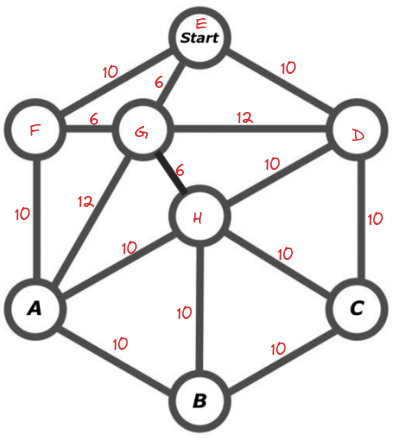
\includegraphics[width=0.95\linewidth]{img/graph_with_weighted_edges.png} 
\caption{Gewichteter Graph}
\label{fig:weighted-graph}
\end{subfigure}
\begin{subfigure}{0.720\textwidth}
\begin{footnotesize}
\begin{verbatim}
Shortest distance from E to A is 18 via path: E -> G -> A
Shortest distance from E to B is 22 via path: E -> G -> H -> B
Shortest distance from E to C is 20 via path: E -> D -> C
Shortest distance from E to D is 10 via path: E -> D
Shortest distance from E to E is 0 via path: E
Shortest distance from E to F is 10 via path: E -> F
Shortest distance from E to G is 6 via path: E -> G
Shortest distance from E to H is 12 via path: E -> G -> H
This calculation took about 0.128ms
\end{verbatim}
\end{footnotesize}
\caption{Skript Ausgabe}
\label{fig:djikstra-test-skript-output}
\end{subfigure}

\caption{Djikstra Algorithmus Test mit Python}
\label{fig:djikstra-test-output}
\end{figure}

Um den kürzesten Pfad achtmal zu berechnen, wurden etwa 0,128 ms benötigt, was ausreichend schnell ist. Aufgrund dieses Tests wurde entschieden, einen selbst implementierten, einfachen Dijkstra-Algorithmus zu verwenden, da es wichtig ist, dass der Algorithmus möglichst leichtgewichtig ist, da nur begrenzte Rechenleistung und Speicher zur Verfügung stehen.

Das Skript wurde in einem Github Gist veröffentlicht und ist unter folgendem Link aufrufbar: \url{https://gist.github.com/dimschlukas/2632116f913b1e10eea9be40e62b2630}

\subsubsection{Kamera Position}\label{camera-position}

Die Platzierung der Kamera ist ein entscheidender Faktor, um sicherzustellen, dass sie die gewünschten Objekte und Bereiche korrekt erfassen kann. Im Folgenden werden die relevanten Parameter erläutert:

\begin{itemize}
    \item Kamera wird auf einer Höhe von 22.5cm montiert.
    \item Field of View der Kamera beträgt 66\textdegree.
    \item Kamera soll Knoten in einer nähe bis zu 15cm vor dem Roboter aufzeichnen.
    \item Kamera soll Objekte bis zu 2 Meter Entfernung aufzeichnen.
\end{itemize}

Nachfolgend skizziert wie diese Parameter die Position und Neigung der Kamera definieren:

\begin{figure}[H]
    \centering
    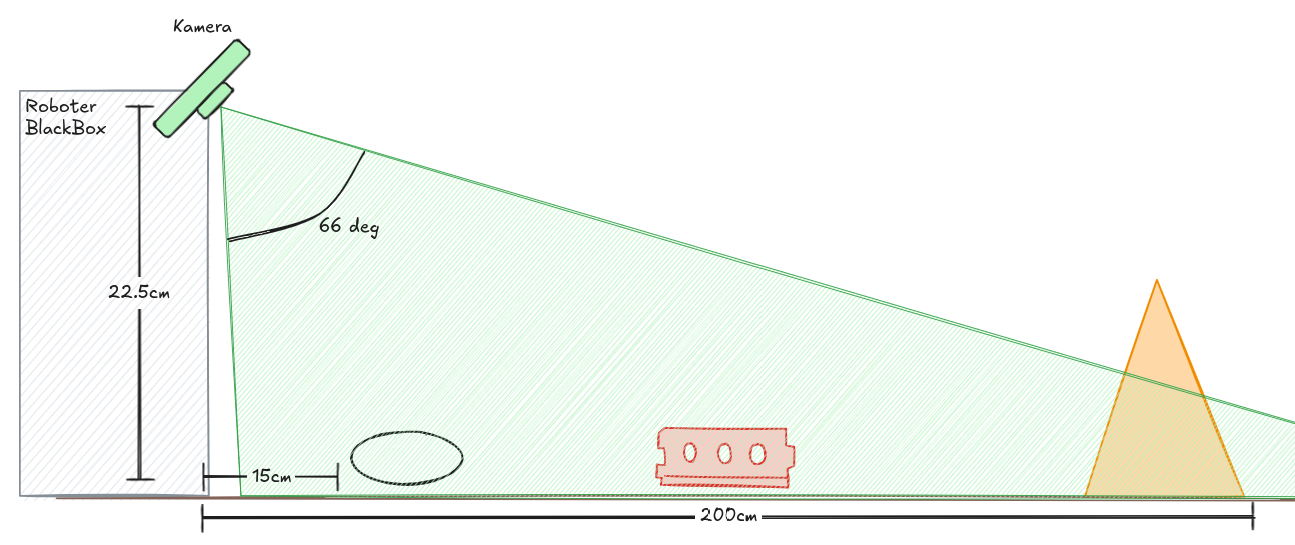
\includegraphics[width=1\linewidth]{assets/informatik-prototyp/camera/camera_position.png}
    \caption{Skizze der Kamera Positionierung}
    \label{fig:camera-position}
\end{figure}

Aus den Parametern kann also berechnet werden, dass die Kamera in einem Winkel von ca. 56\textdegree\ eingebaut werden muss. Um die Knoten in der nähe sowie die Pylonen in der Distanz zu erfassen:

Nachfolgend dies dargestellt in einem Graphen mit korrekten Proportionen:

\begin{figure}[H]
    \centering
    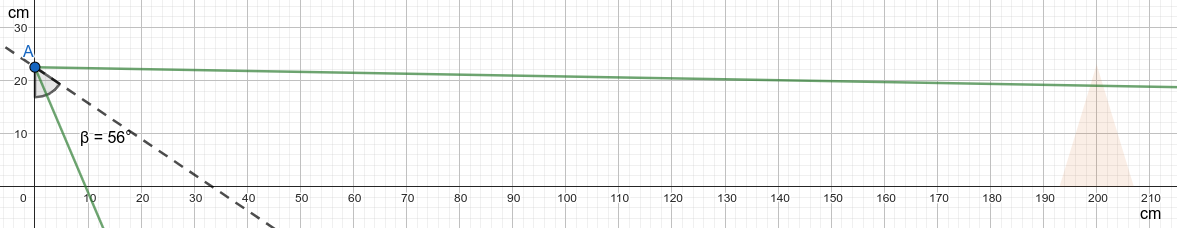
\includegraphics[width=1\linewidth]{assets/informatik-prototyp/camera/camera_position_exact_bigger.png}
    \caption{Graph der Kamera Positionierung}
    \label{fig:camera-position-exact}
\end{figure}

Zusätzlich haben wir dies mit unserem Raspberry und Kamera nachgestellt:

\begin{figure}[H]
\centering
\begin{subfigure}{0.45\textwidth}
\centering
    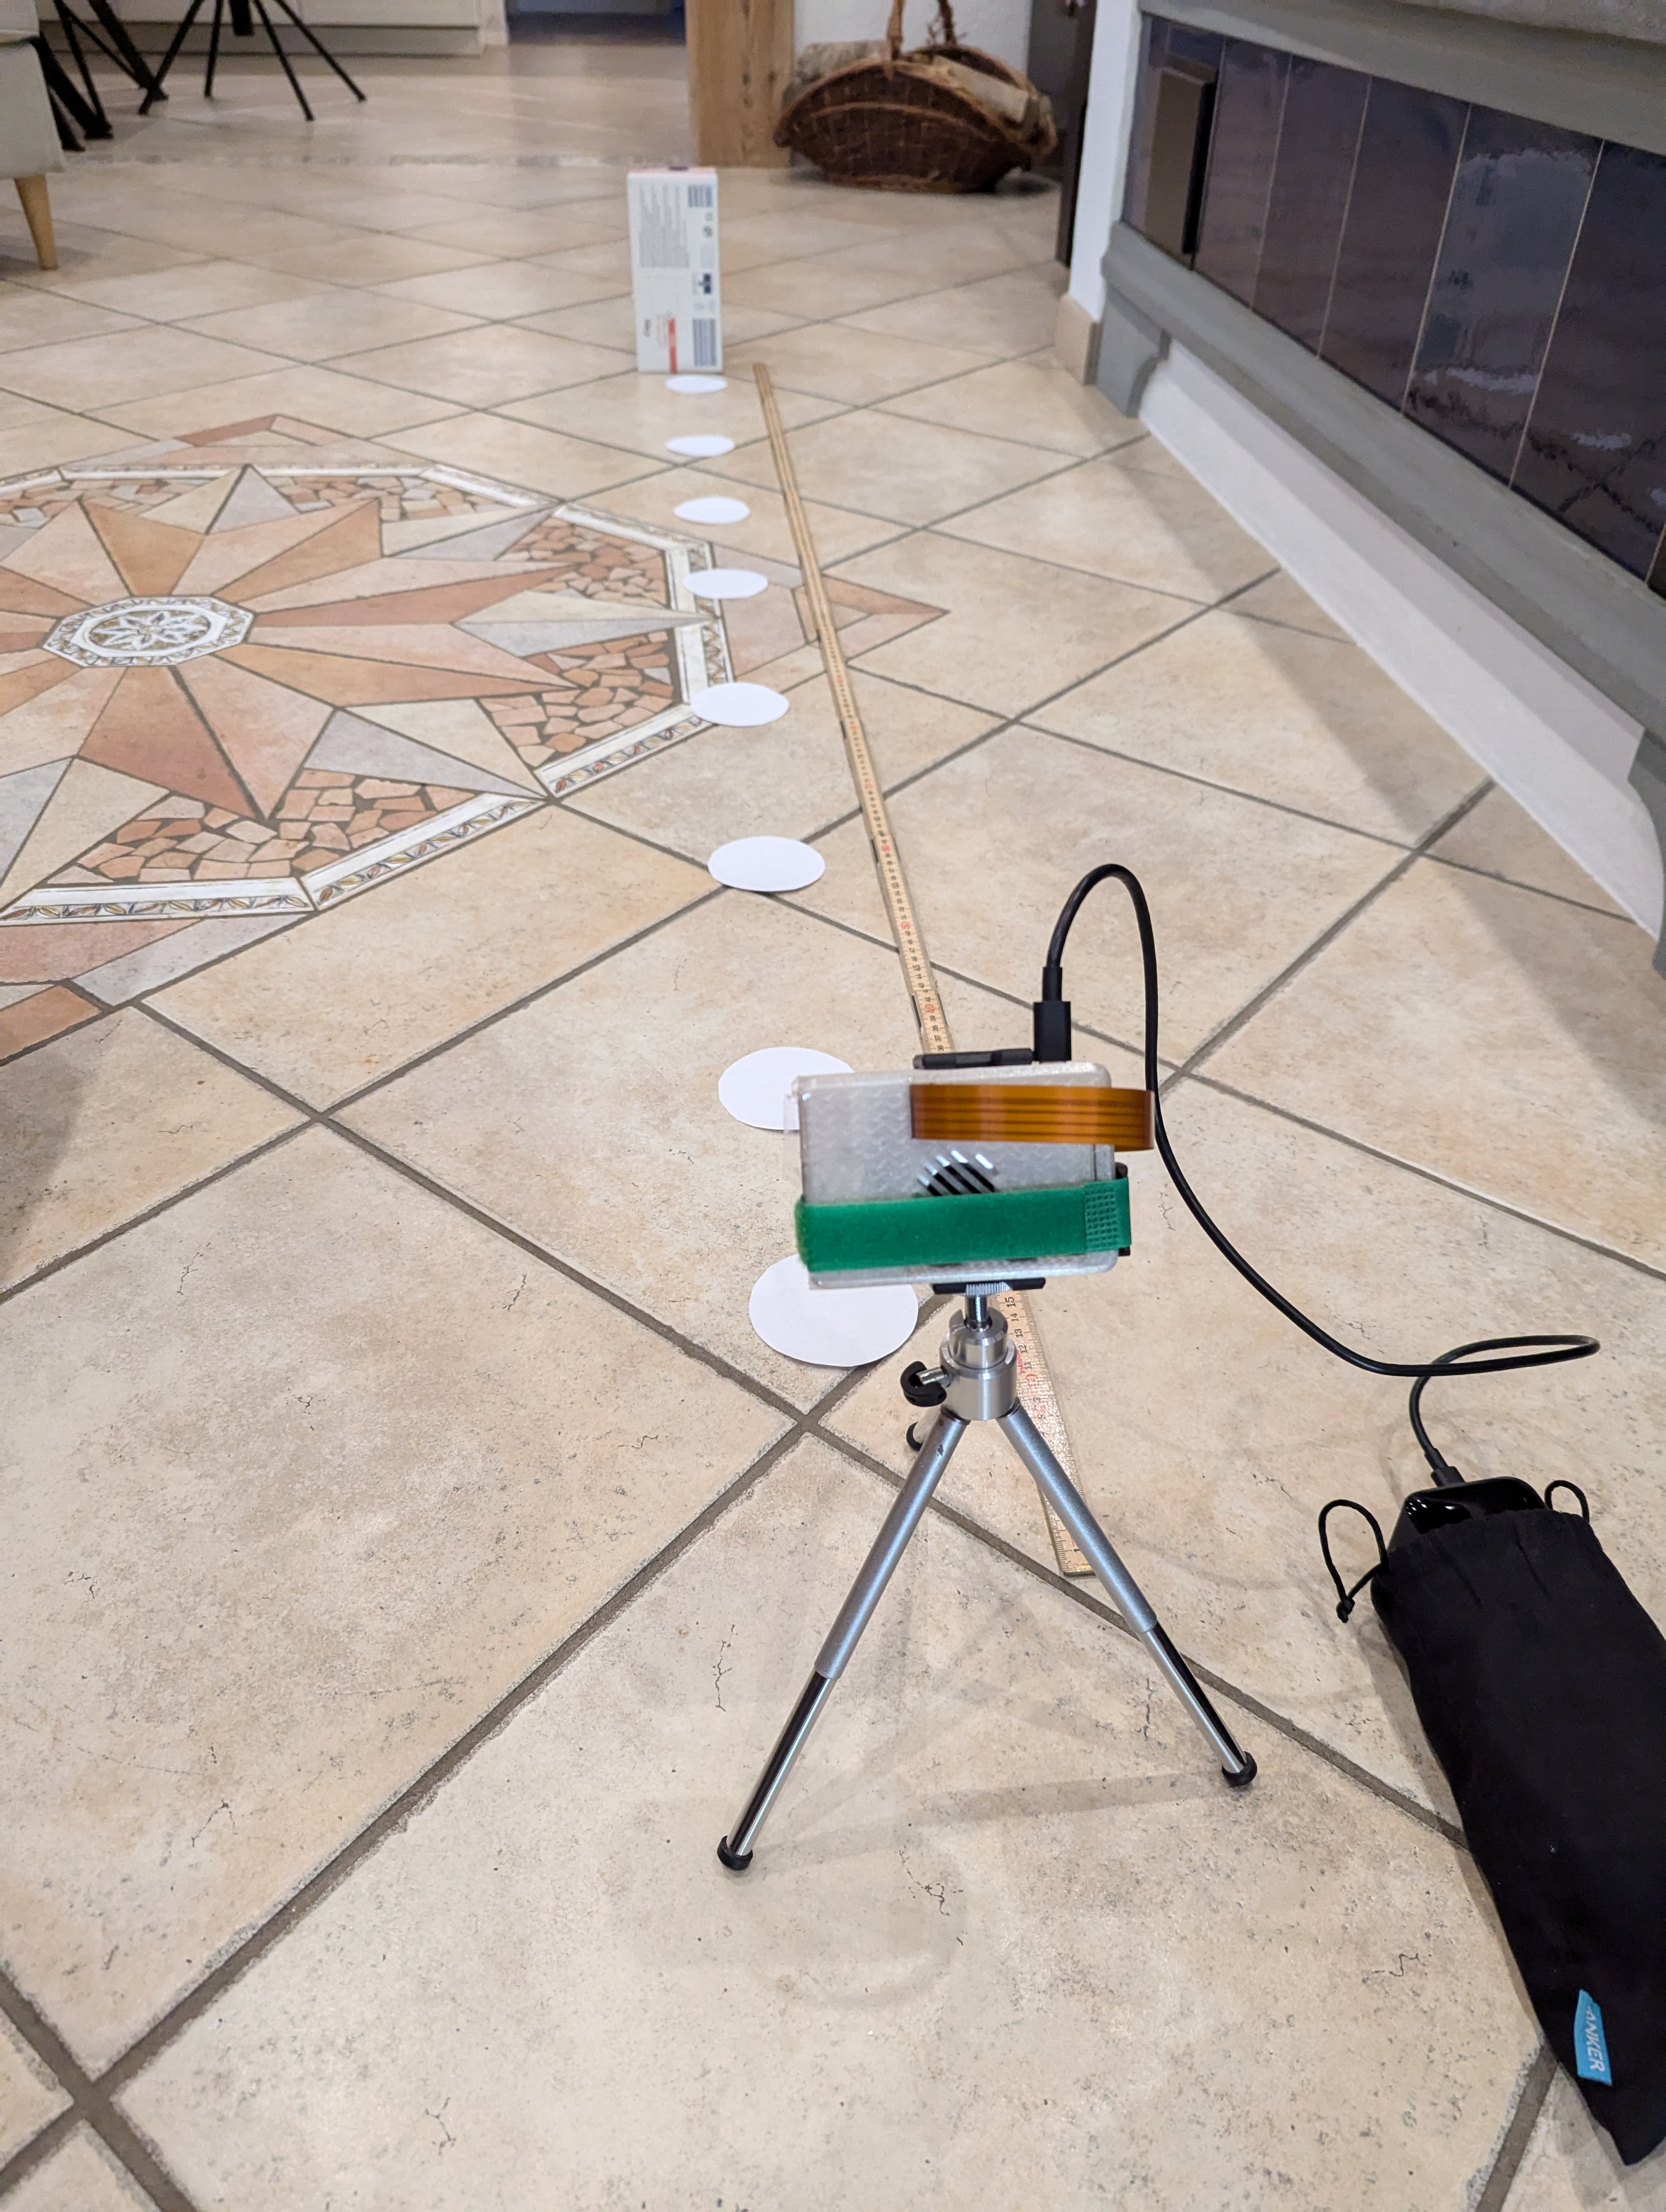
\includegraphics[height=7cm]{assets/informatik-prototyp/camera/camera_position_prototype_at_home.jpg}
\end{subfigure}
\begin{subfigure}{0.45\textwidth}
\centering
    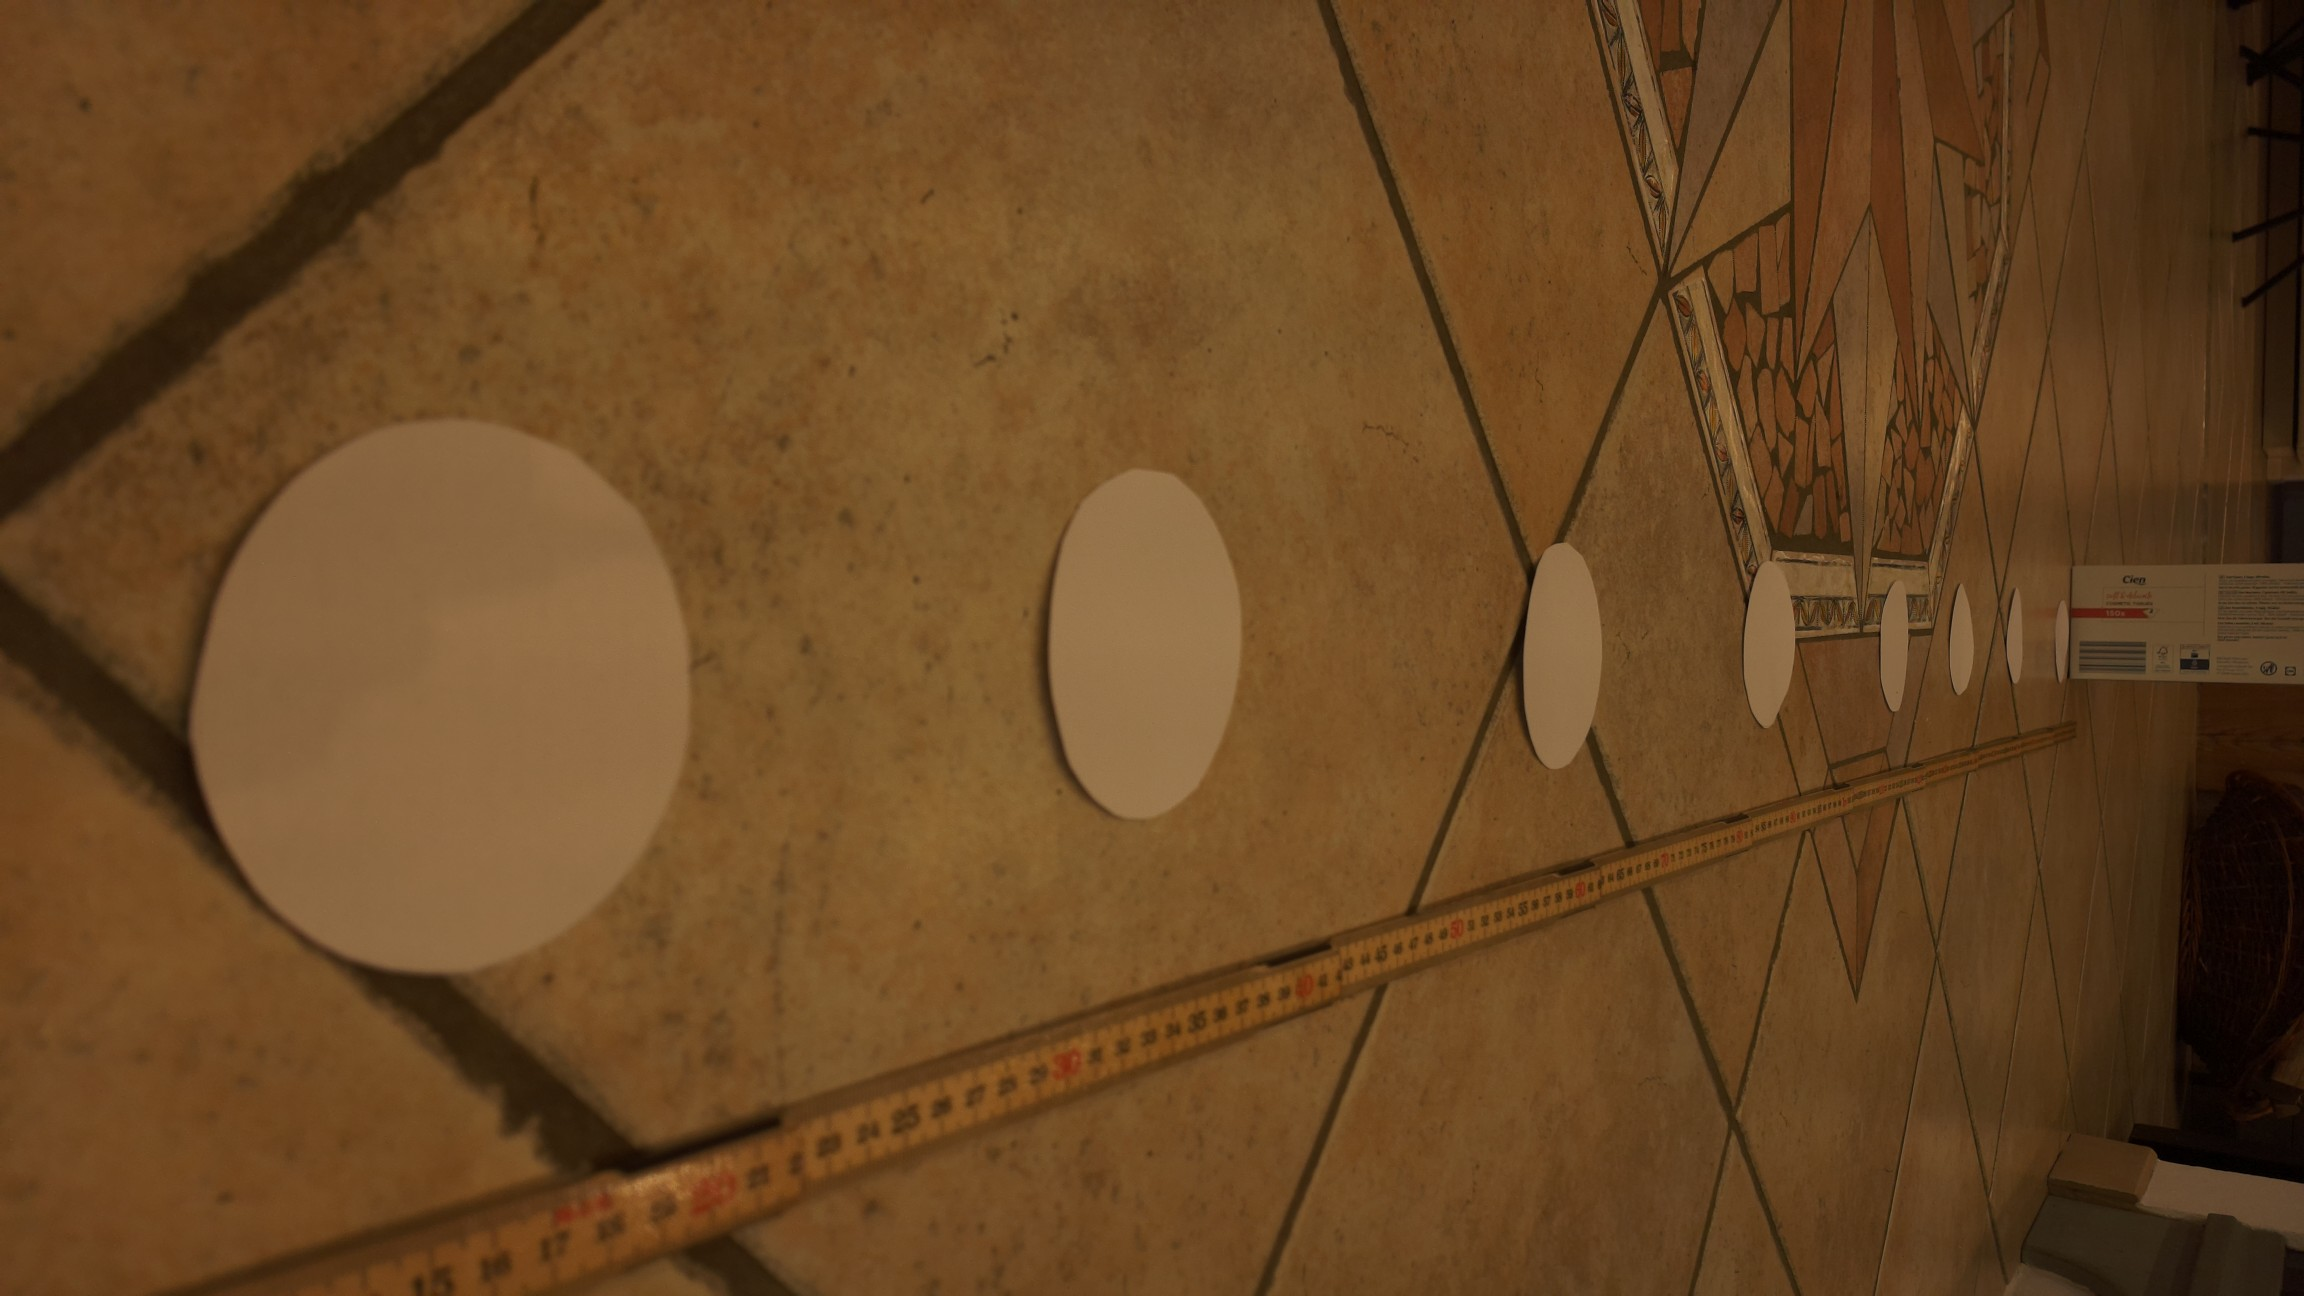
\includegraphics[height=7cm]{assets/informatik-prototyp/camera/camera_position_prototype.jpg}
\end{subfigure}
\caption{Test der Kamera Position}
\label{fig:camera-position-prototype}
\end{figure}


\subsubsection{Winkelerkennung}\label{winkelerkennung}

Um die Winkel der abgehenden Kanten eines Knoten zu detektieren, macht unser Roboter vor dem Befahren eines Knotens ein Bild dessen. Dazu ist jedoch zu beachten, wie in Kapitel \ref{camera-position} beschrieben, wird unsere Kamera in einem Winkel von 56\textdegree\ montiert. So können wir naheliegende Knoten vor dem Roboter, wie auch weit entfernte Pylonen in einem Bild erkennen, ohne die Kamera schwenken zu müssen.
Da wir dadurch nun aber verzerrte Bilder aufzeichnen, muss an dem Bild zuerst eine geometrische Transformation durchgeführt werden. Sodass wir schlussendlich ein verzerrungsfreihe Ansicht auf den Knoten haben. Anschliessend können die einzelnen Winkel ohne Probleme durch maskieren und detektieren von Formen mittels Opencv berechnet werden.

Nachfolgend wird dies Schritt für Schritt nachvollziehbar dargestellt:

\begin{enumerate}
    \item Vor dem Knoten anhalten und Bild aufnehmen
    % \begin{figure}[H]
    %     \centering
    %     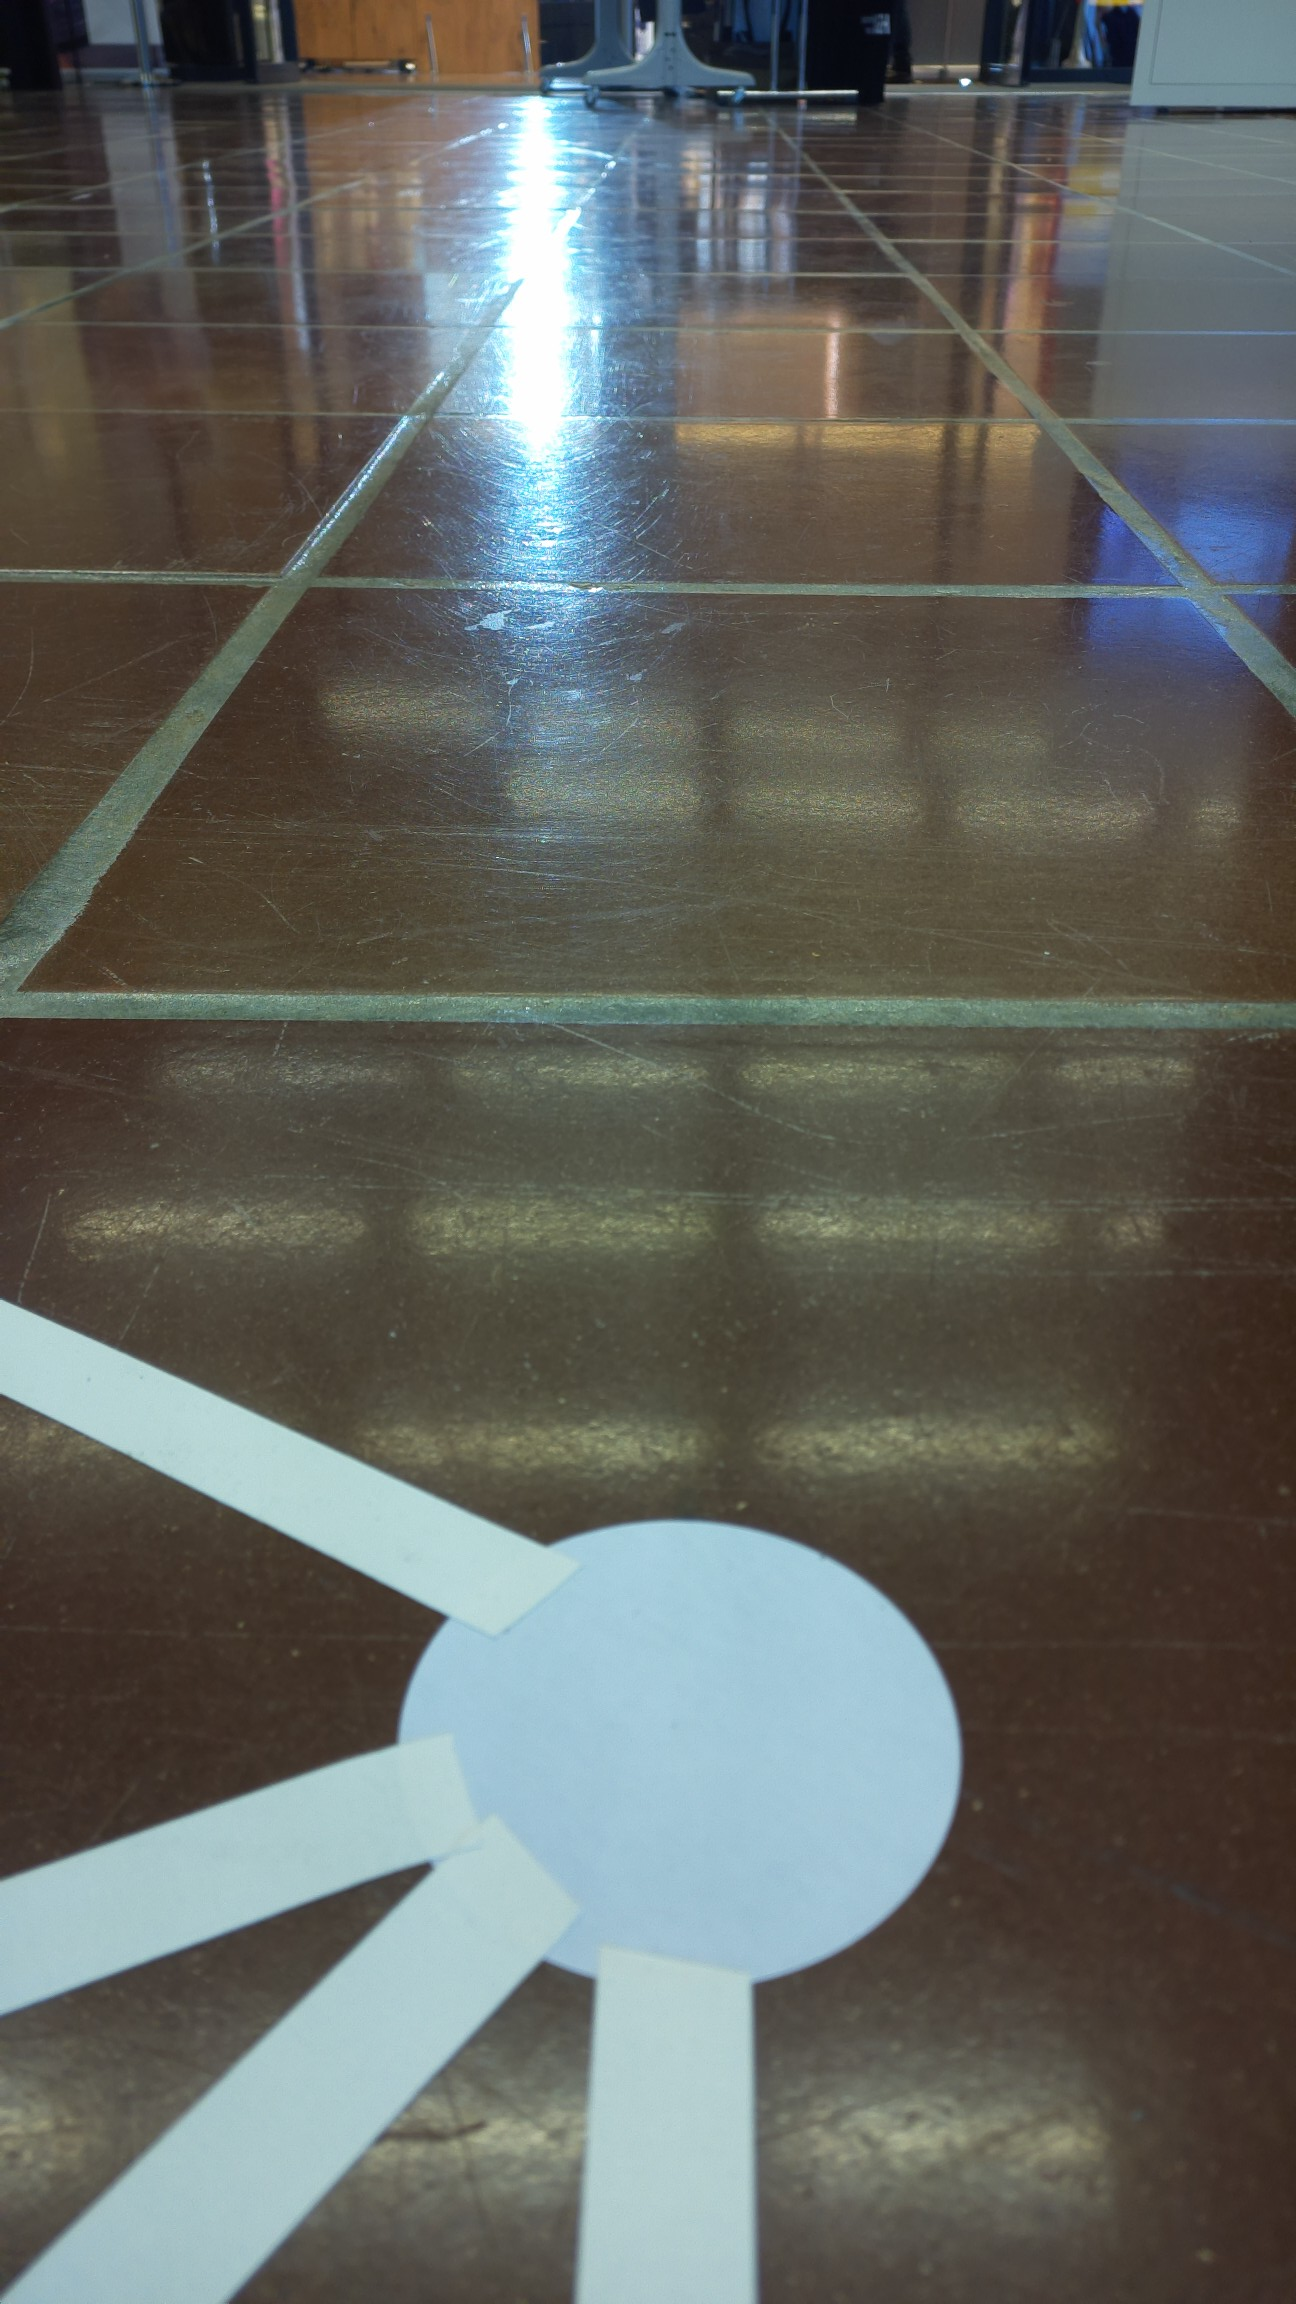
\includegraphics[width=0.5\linewidth]{assets/informatik-prototyp/opencv/angle_detection/image_taken_by_pi_camer_before_node.jpg}
    %     \caption{Originale Kamera Aufnahme eines Knotens}
    %     \label{fig:before-node}
    % \end{figure}


    \begin{figure}[H]
        \centering
        \begin{subfigure}{0.25\textwidth}
        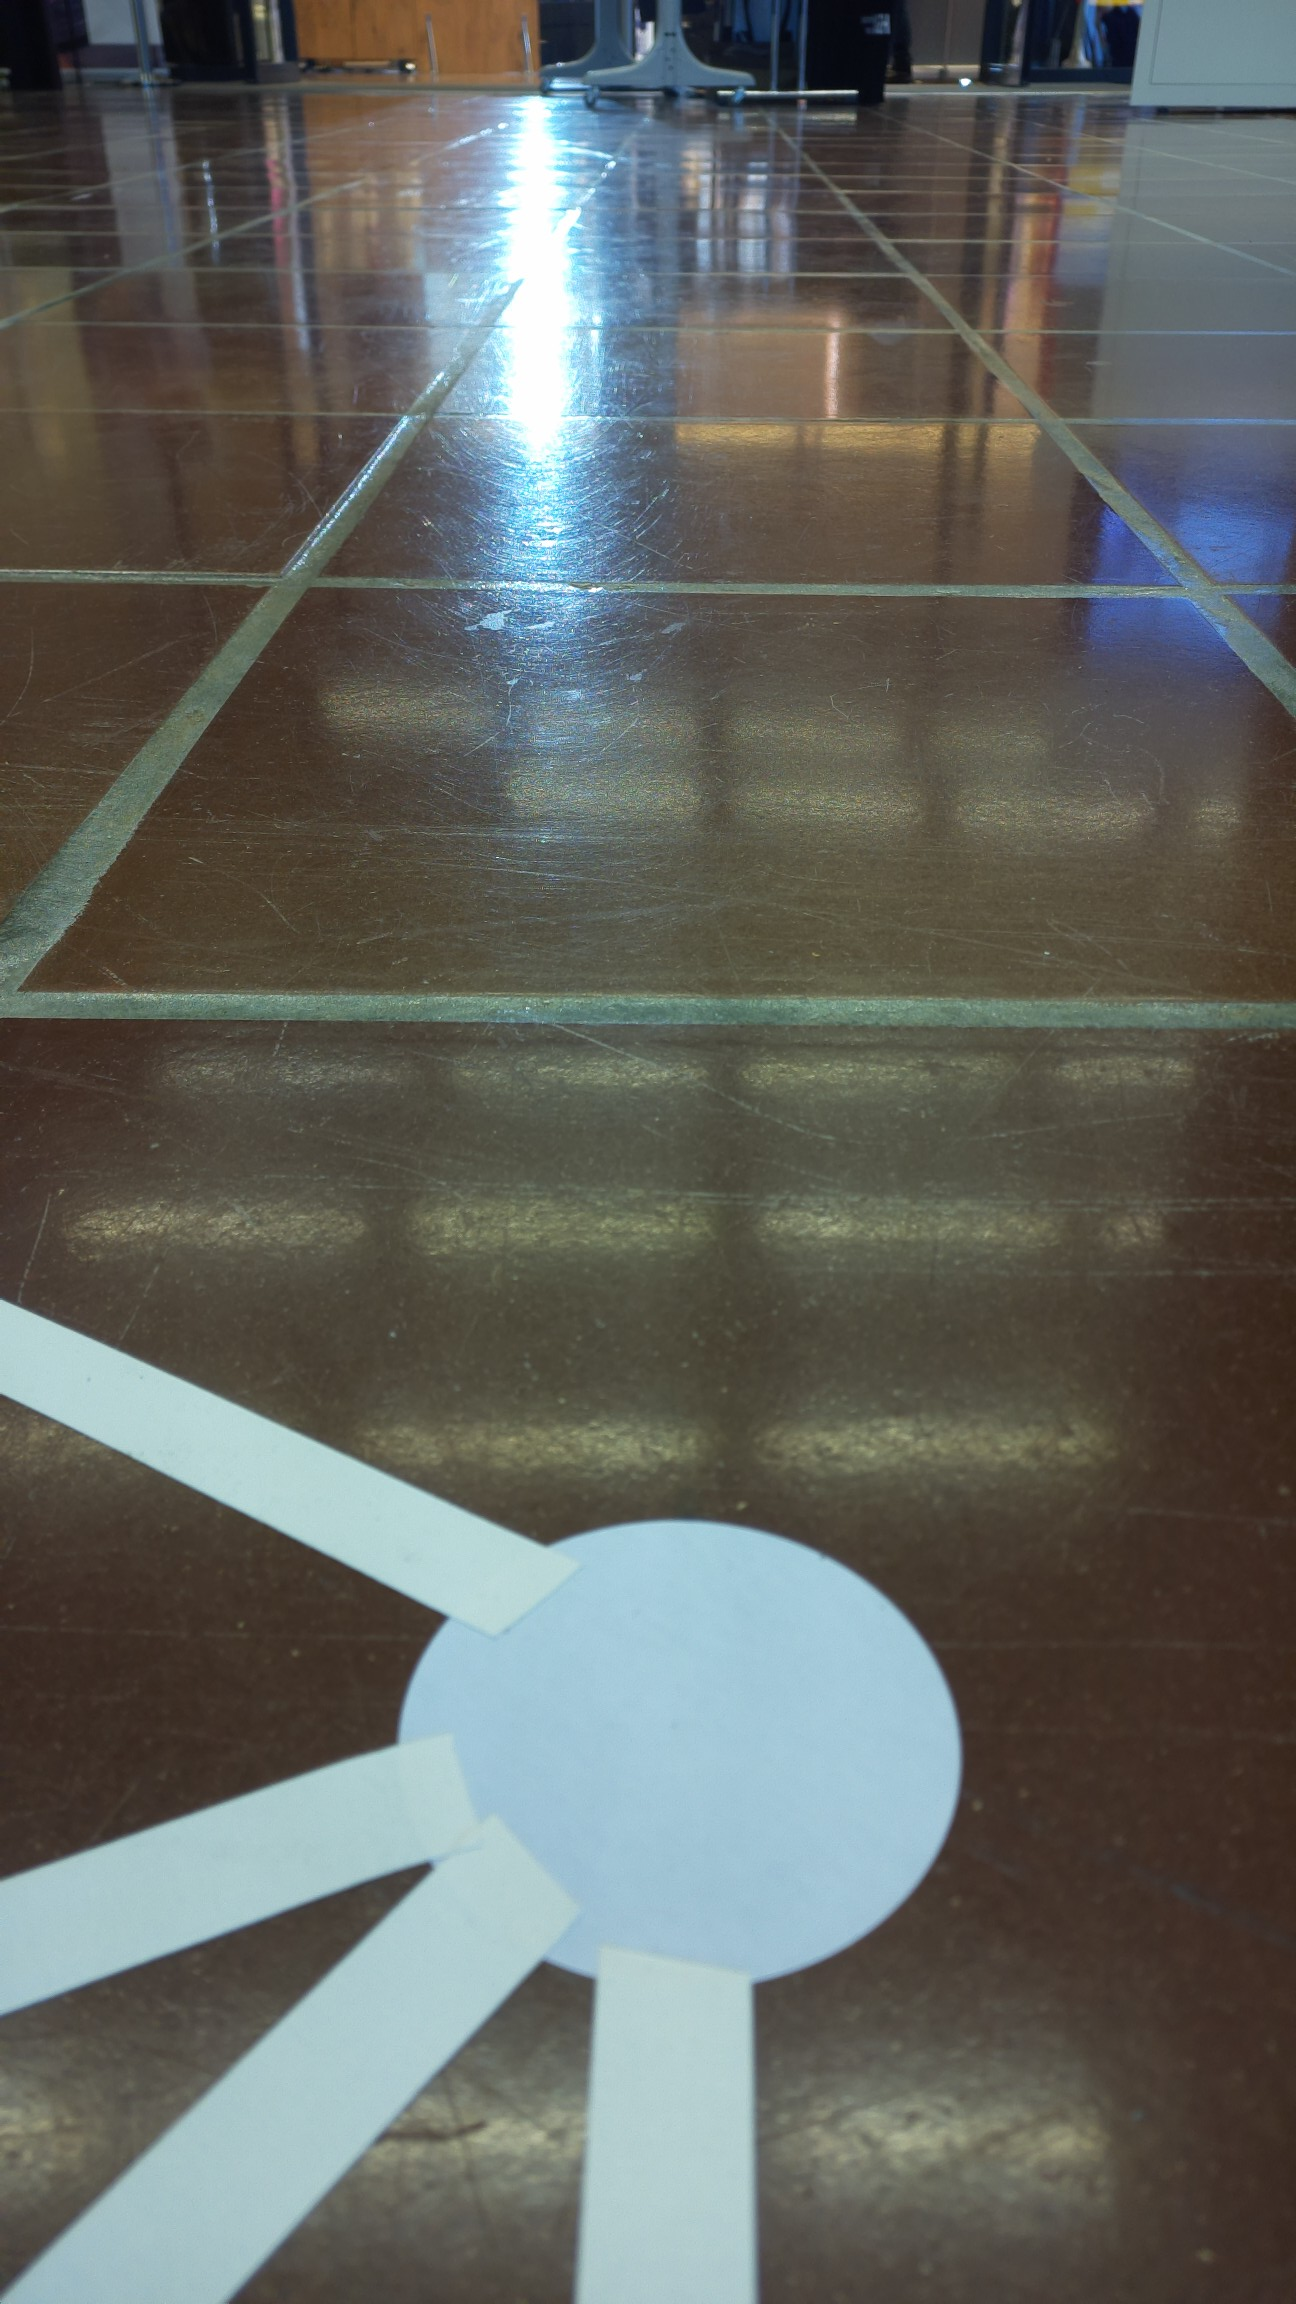
\includegraphics[width=0.95\linewidth]{assets/informatik-prototyp/opencv/angle_detection/image_taken_by_pi_camer_before_node.jpg}
        \caption{Originale Kamera Aufnahme eines Knotens}
        \label{fig:before-node}
        \end{subfigure}
        \begin{subfigure}{0.5\textwidth}
        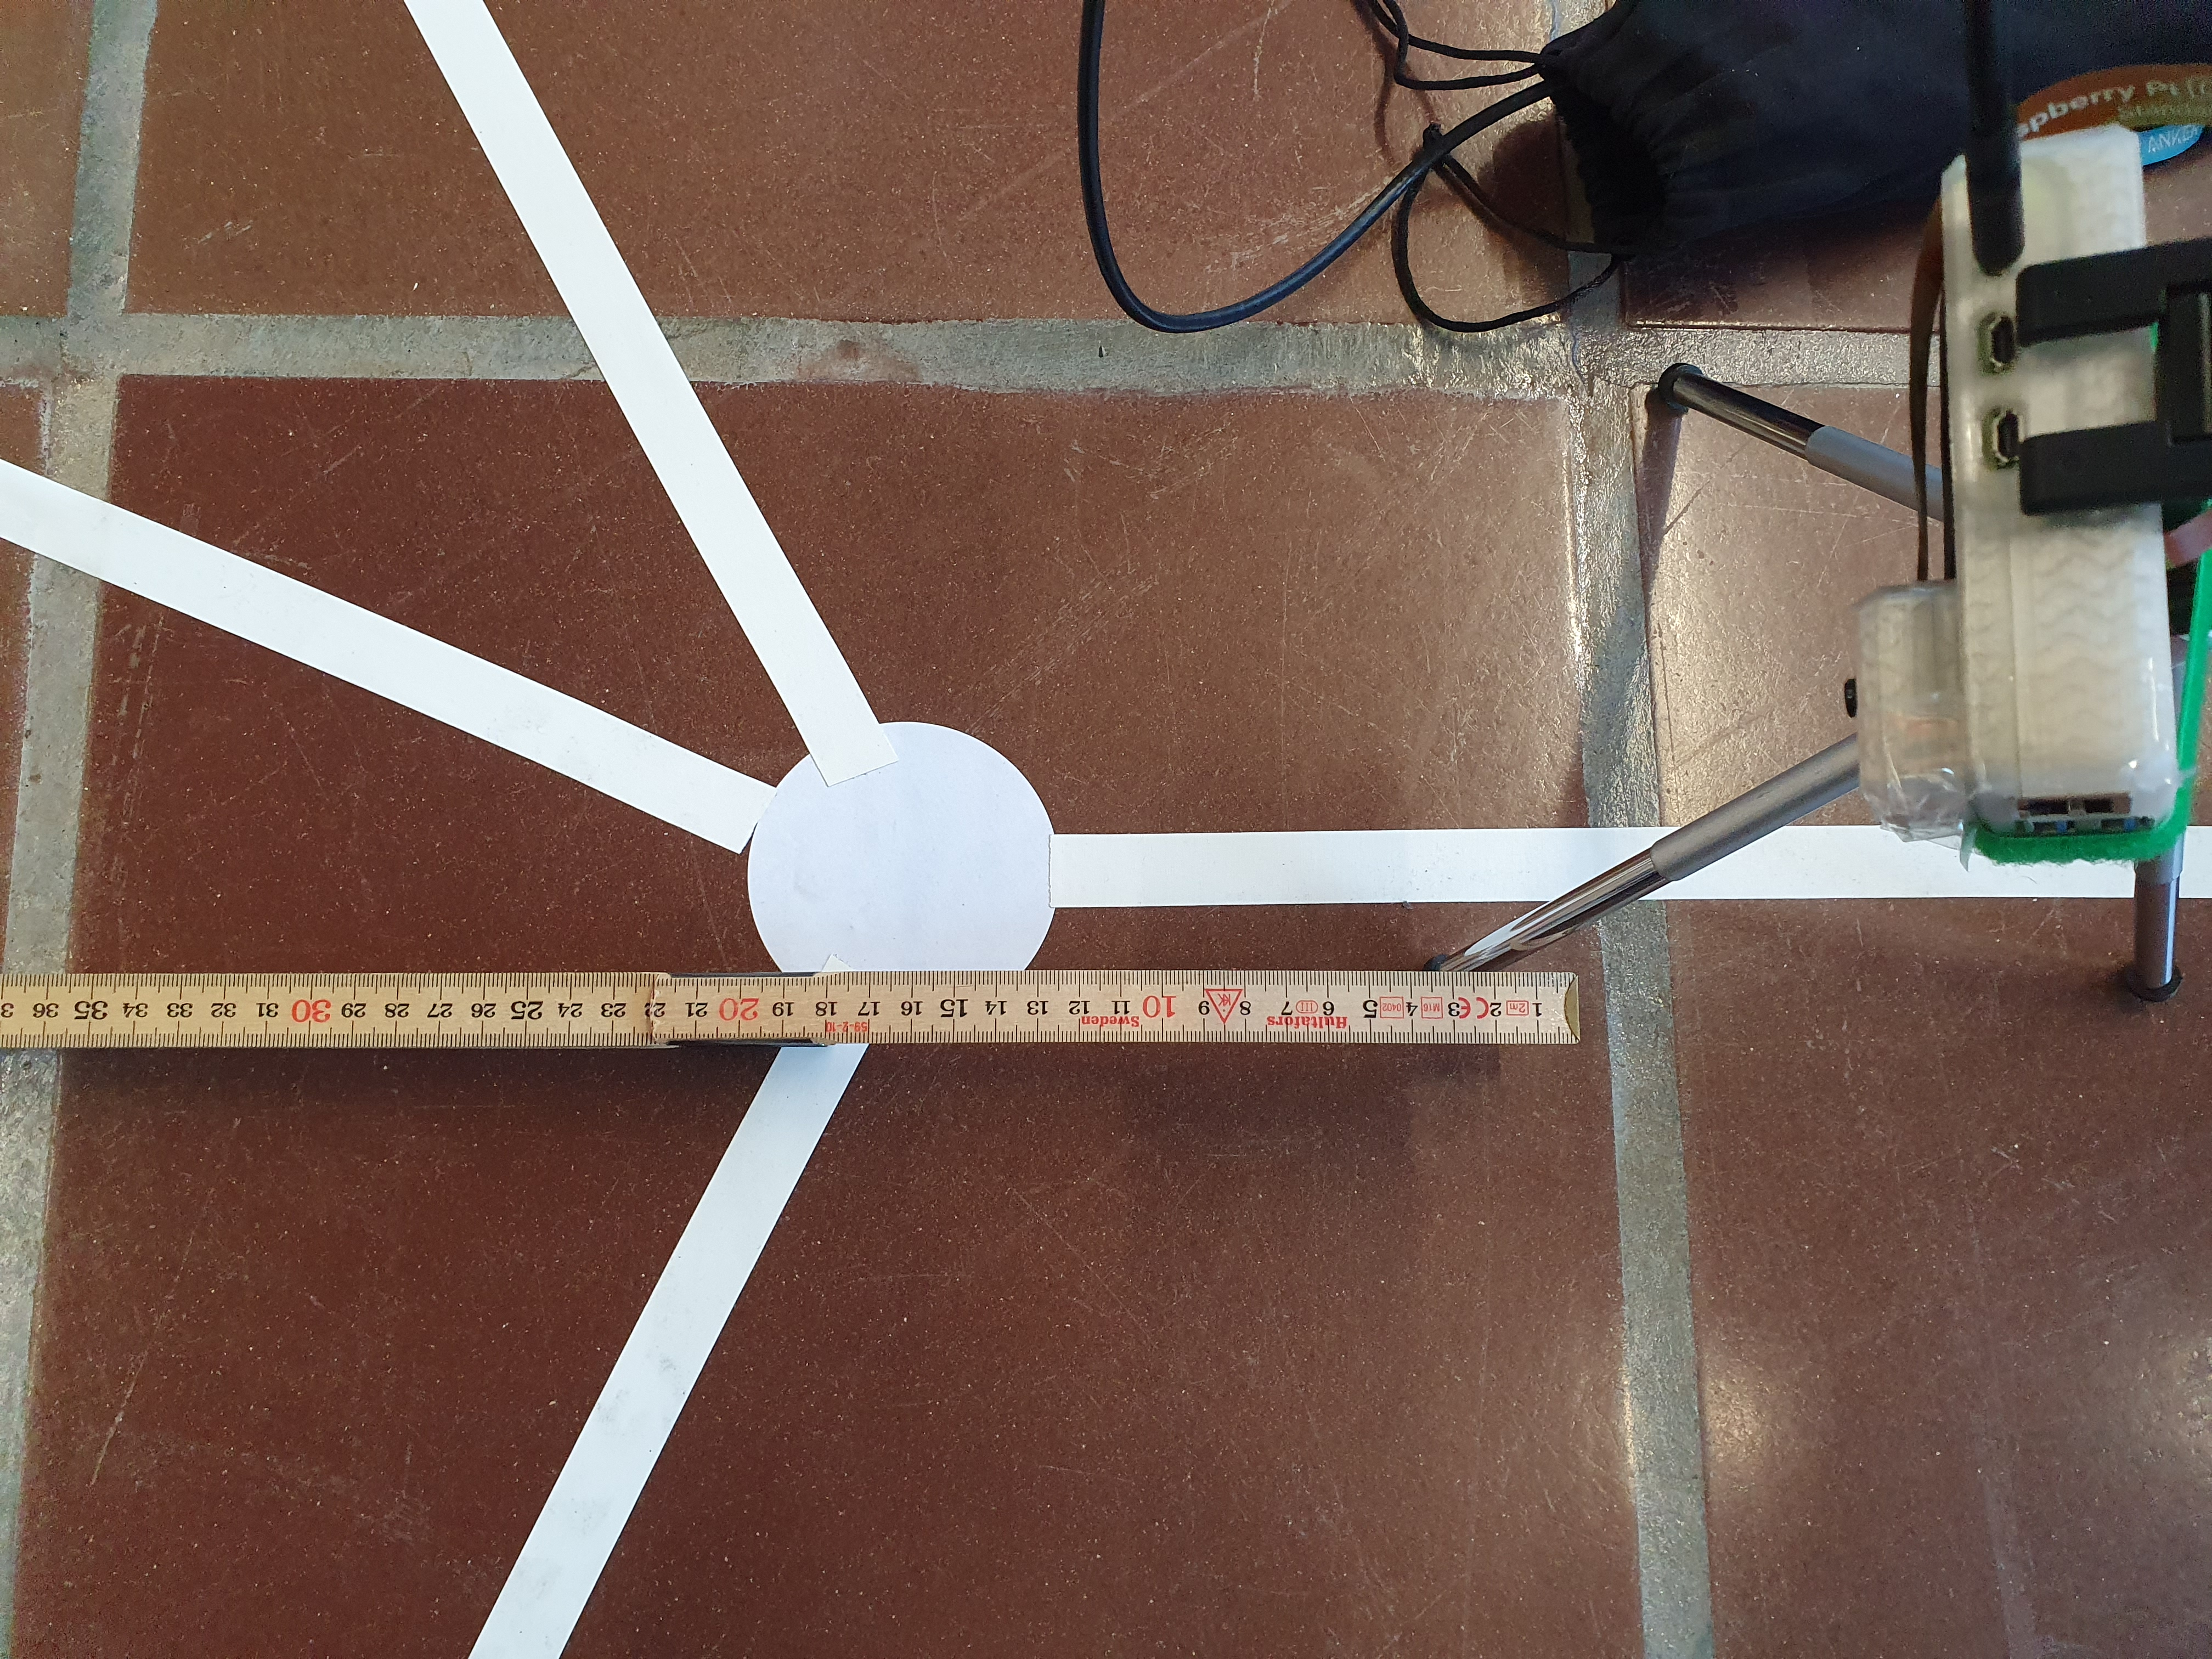
\includegraphics[width=0.95\linewidth]{assets/informatik-prototyp/opencv/camera_position_before_node.jpg} 
        \caption{Kamera vor Knoten}
        \label{fig:before-node-camera}
        \vspace{5mm}
        \end{subfigure}
        \caption{Aufnahme vor Knoten}
        \label{fig:image-before-node}
        \end{figure}

        
    \item Geometrische Transformation anhand fix definierten Punkten anwenden
        \begin{figure}[H]
        \centering
        \begin{subfigure}{0.4\textwidth}
        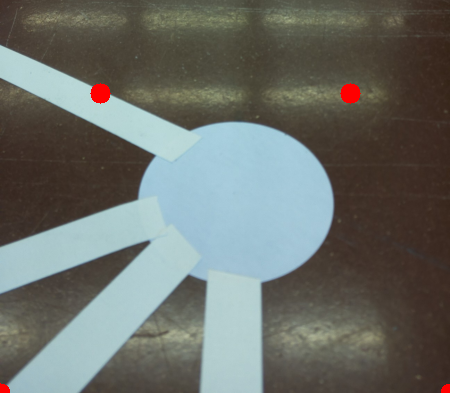
\includegraphics[width=0.95\linewidth]{assets/informatik-prototyp/opencv/angle_detection/node_before_transformation_corners.png} 
        \caption{Vier Punkte für Transformation}
        \label{fig:node-before-geometric-transform}
        \end{subfigure}
        \begin{subfigure}{0.4\textwidth}
        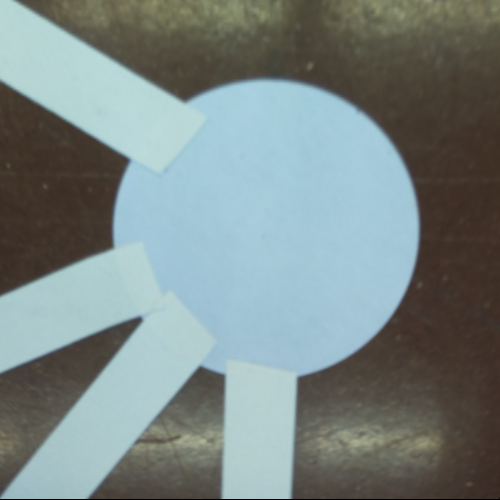
\includegraphics[width=0.95\linewidth]{assets/informatik-prototyp/opencv/angle_detection/node_after_transformation.png} 
        \caption{Nach Transformation}
        \label{fig:node-after-geometric-transform}
        \end{subfigure}
        \caption{Geometrische Transformation}
        \label{fig:node-geometric-transform}
        \end{figure}
    \item Knoten maskieren und dessen Mittelpunkt detektieren
        \begin{figure}[H]
        \centering
        \begin{subfigure}{0.4\textwidth}
        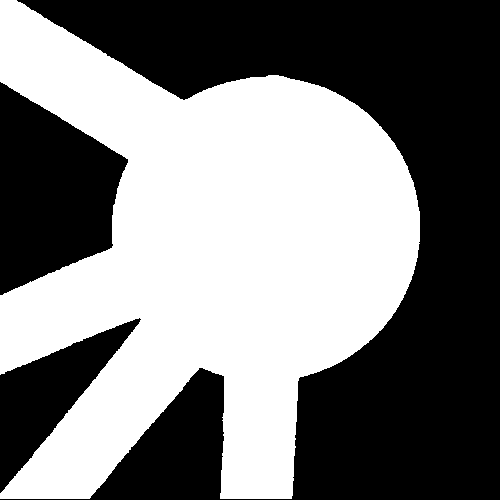
\includegraphics[width=0.95\linewidth]{assets/informatik-prototyp/opencv/angle_detection/node_after_transformation_masked.png} 
        \caption{Maskieren}
        \label{fig:node-masked}
        \end{subfigure}
        \begin{subfigure}{0.4\textwidth}
        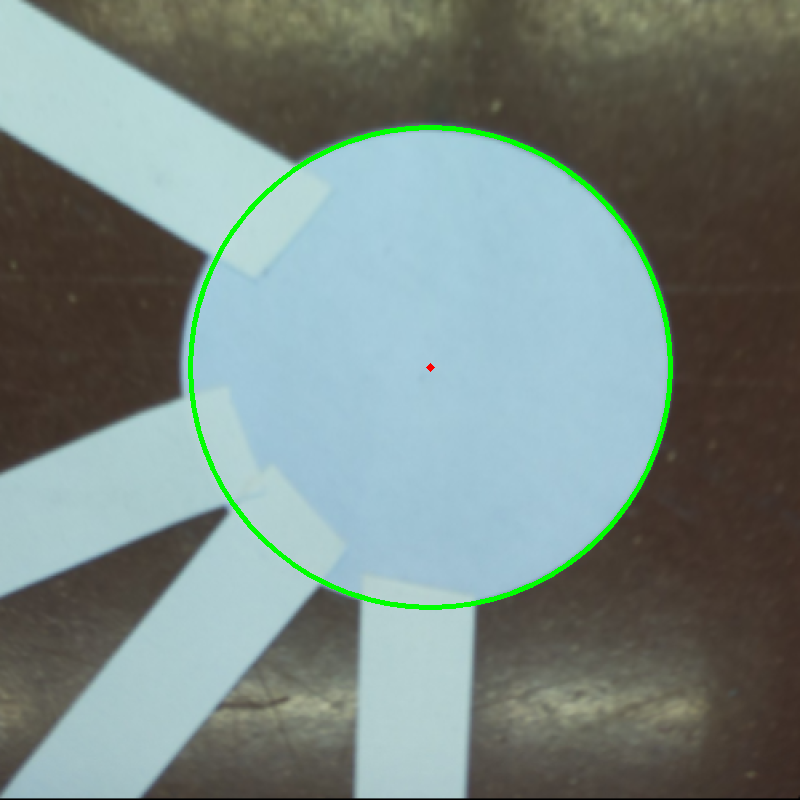
\includegraphics[width=0.95\linewidth]{assets/informatik-prototyp/opencv/angle_detection/node_detecting_center.png} 
        \caption{Mittelpunkt des Knoten detektieren}
        \label{fig:node-center}
        \end{subfigure}
        \caption{Knoten und dessen Mittelpunkt detektieren}
        \label{fig:detecting-node}
        \end{figure}
    \item Ausgehende Kanten maskieren
        \begin{figure}[H]
        \centering
        \begin{subfigure}{0.4\textwidth}
        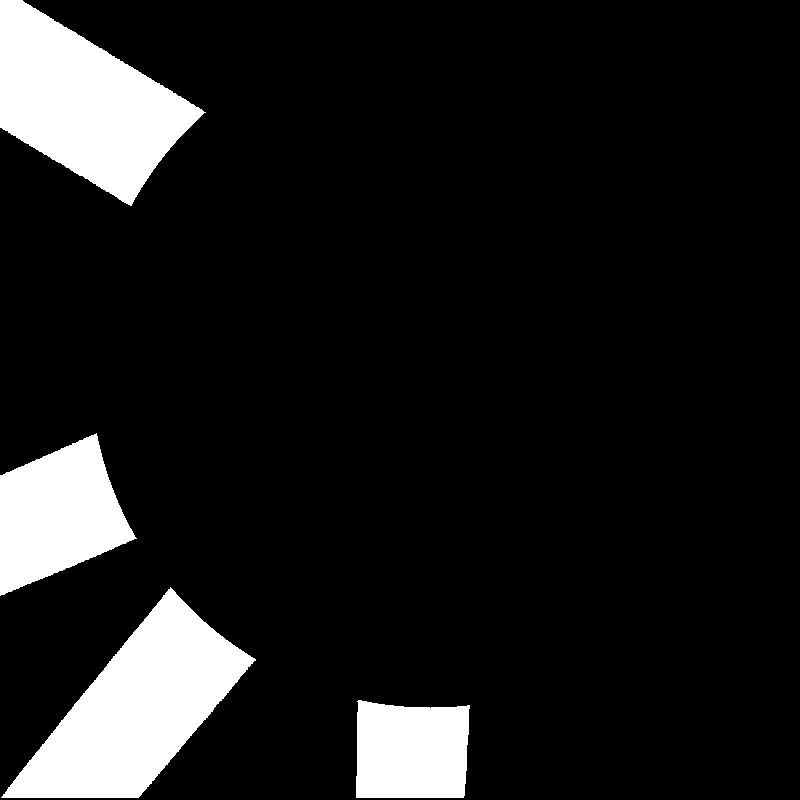
\includegraphics[width=0.95\linewidth]{assets/informatik-prototyp/opencv/angle_detection/edge_masked.png} 
        \caption{Nur Kanten maskieren}
        \label{fig:edge-masked}
        \end{subfigure}
        \begin{subfigure}{0.4\textwidth}
        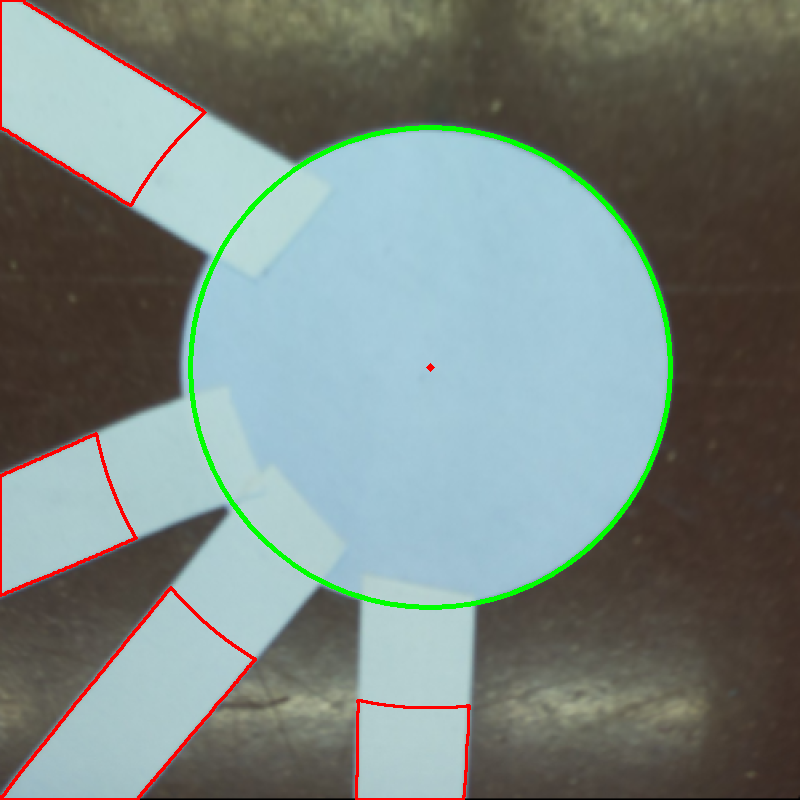
\includegraphics[width=0.95\linewidth]{assets/informatik-prototyp/opencv/angle_detection/edge_contours.png} 
        \caption{Kontur der Kanten zeichnen}
        \label{fig:edge-contours}
        \end{subfigure}
        \caption{Kanten detektieren}
        \label{fig:detecting-edges}
        \end{figure}
    \item Geometrischer Schwerpunkt der Kanten berechnen und Winkel zu Knoten Zentrum berechnen.
        \begin{figure}[H]
        \centering
        \begin{subfigure}{0.4\textwidth}
        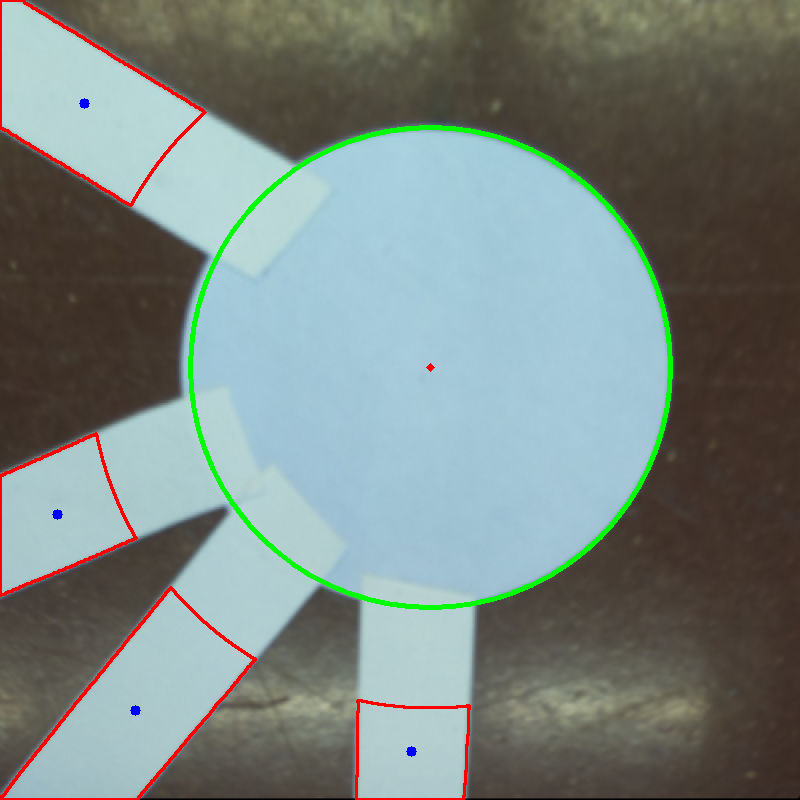
\includegraphics[width=0.95\linewidth]{assets/informatik-prototyp/opencv/angle_detection/edge_detect_centers.png} 
        \caption{Mittelpunkte der Kanten berechnen}
        \label{fig:edge-center}
        \end{subfigure}
        \begin{subfigure}{0.4\textwidth}
        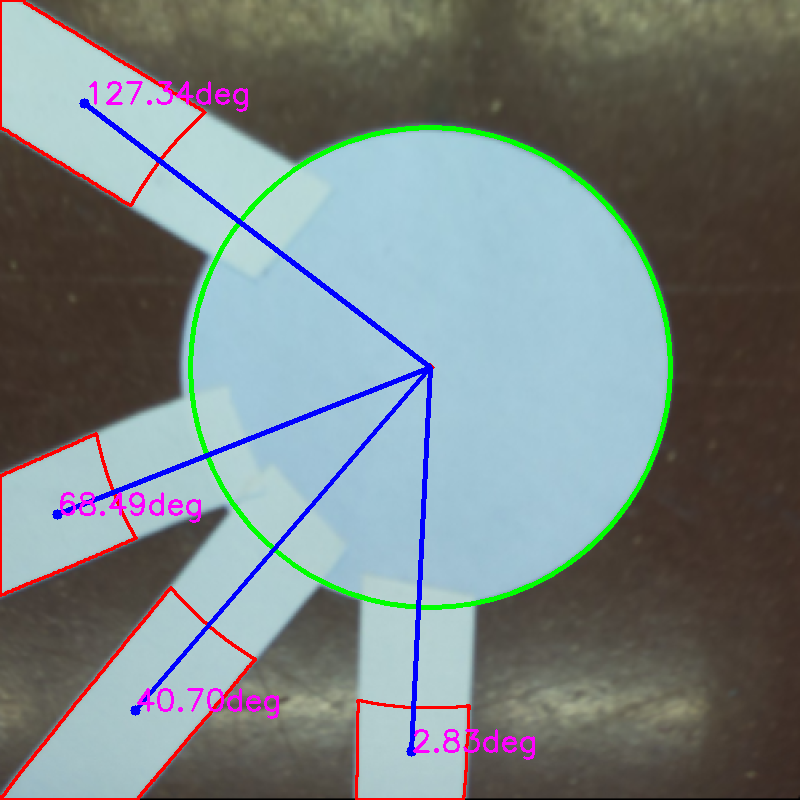
\includegraphics[width=0.95\linewidth]{assets/informatik-prototyp/opencv/angle_detection/node_with_edge_angles_annotated.png} 
        \caption{Winkel der Kanten}
        \label{fig:angle-lines}
        \end{subfigure}
        \caption{Winkel der einzelnen Kanten detektieren}
        \label{fig:node-with-edge-angles}
        \end{figure}
\end{enumerate}

\subsubsection{Graph-, Pylonen- und Barriere-Erkennung}



% \textbf{Spiegelung}

% Starke Spiegelungen stellen ein grosses Problem bei der Erkennung von Knoten dar. Um die Bilder zu entspiegeln, können die Lichtverhältnisse angepasst, Polfilter verwendet oder Nachbearbeitungen durchgeführt werden.\cite{avoid-reflection}

% Beleuchtung

Als Basis für die Bilderkennung, wurde ein Graph aufgeklebt in der Mensa (Abb. \ref{fig:test-graph}). Es wurden mehrere Bilder gemacht, wobei Pylonen und Barrieren willkürlich auf Knoten und Kanten gestellt wurden und immer wieder verschoben wurden.

\begin{figure}[H]
    \centering
    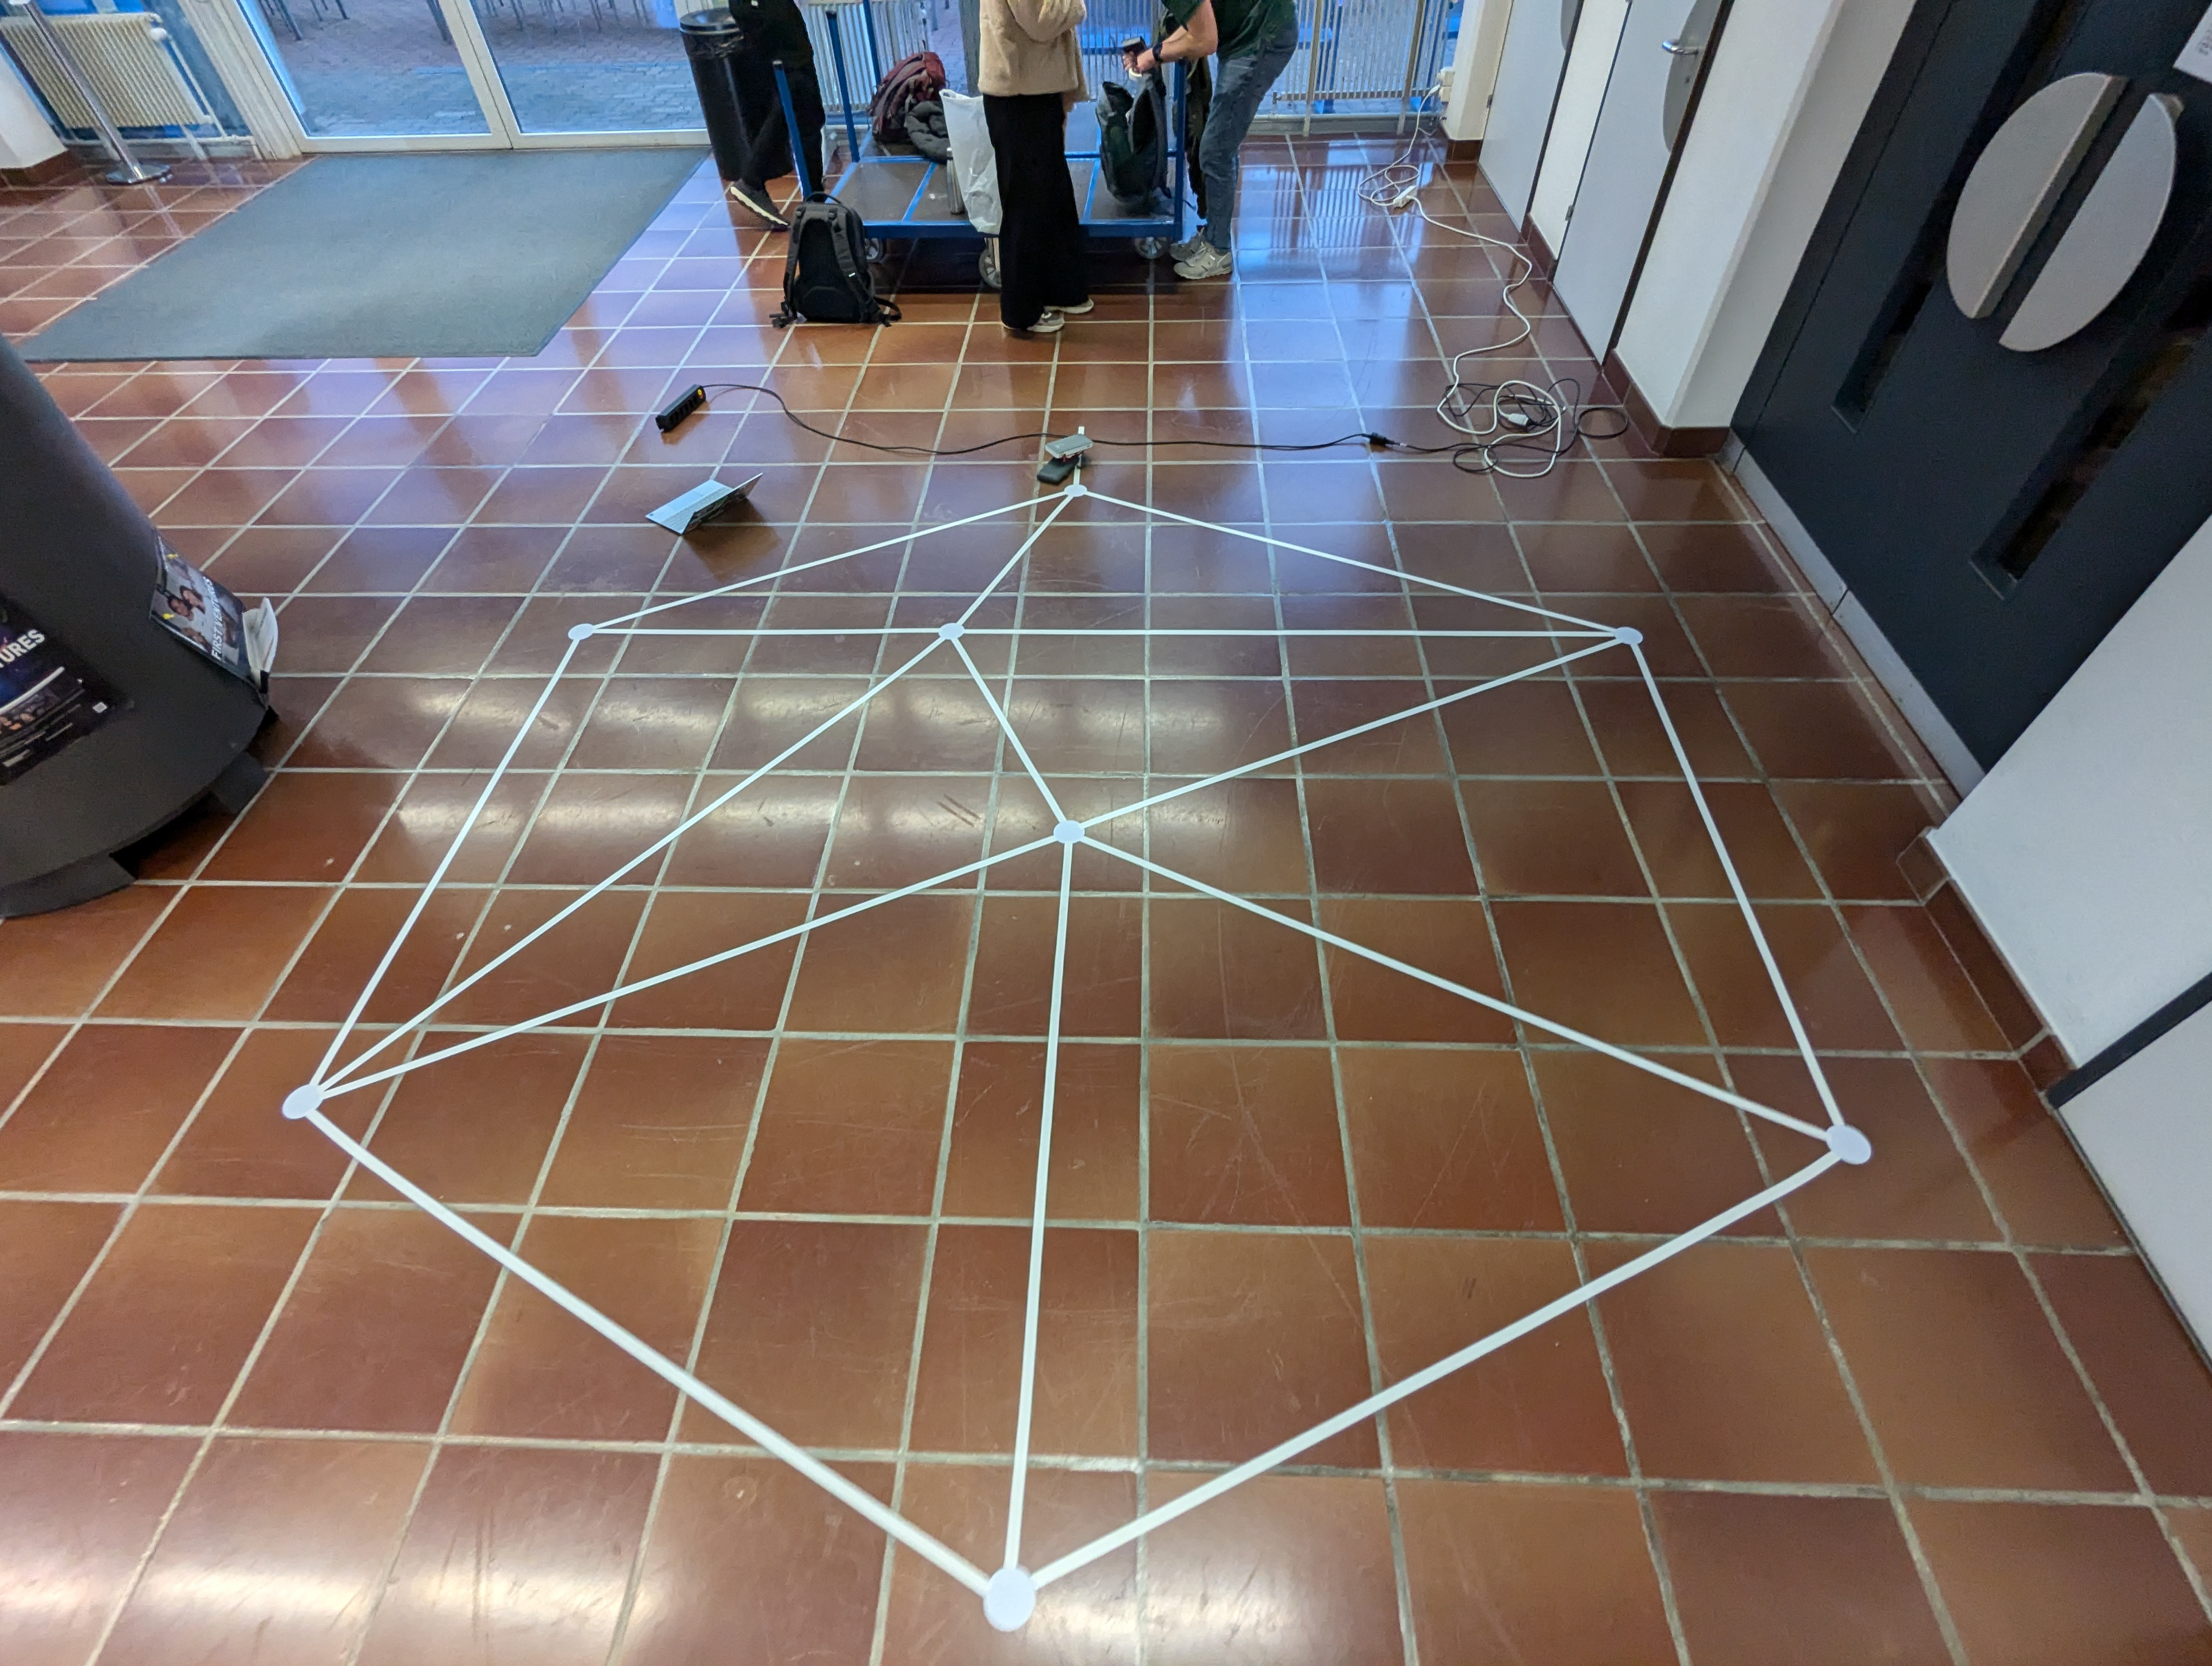
\includegraphics[width=1\linewidth]{assets/informatik-prototyp/opencv/test_graph.jpg}
    \caption{Aufgeklebter Graph zu Testzwecken}
    \label{fig:test-graph}
\end{figure}

\textbf{OpenCV SIFT, FAST, ORB Algorithmen}

OpenCV bietet verschiedene Algorithmen zur Merkmalsdetektion und -beschreibung, die in der Bildverarbeitung und Computer Vision zu Objekterkennung und -tracking eingesetzt werden:

\begin{enumerate}
    \item SIFT (Scale-Invariant Feature Transform)
    
    SIFT ist ein Algorithmus, der robuste und skalierungsinvariante Merkmale in Bildern erkennt. Er findet markante Punkte, sogenannte Keypoints, und berechnet Deskriptoren, die invariant gegenüber Skalierung, Rotation und Beleuchtung sind. Es eignet sich gut für Objektwiedererkennung und Bildregistrierung.

    \item FAST (Features from Accelerated Segment Test)
    
    FAST ist ein sehr schneller Eckendetektor, der besonders für Echtzeitanwendungen geeignet ist. Er überprüft, ob ein Pixel ein Merkmal (Ecke) ist, indem es die Intensitäten der Pixel in einem kreisförmigen Muster um es herum vergleicht. Es ist jedoch nicht robust gegenüber Skalierung oder Rotation.

    \item ORB (Oriented FAST and Rotated BRIEF)
    
    ORB kombiniert FAST für die Merkmalsdetektion und BRIEF (Binary Robust Independent Elementary Features) für die Merkmalsbeschreibung. Es erweitert FAST, indem es Orientierung und Rotation berücksichtigt, und bietet eine effiziente, patentfreie Alternative zu SIFT und SURF, mit ähnlicher Genauigkeit und deutlich besserer Performance.
\end{enumerate}

Zusammenfassend:

\begin{itemize}
    \item SIFT ist genau und robust, aber rechenintensiv.
    \item FAST ist schnell, aber weniger robust.
    \item ORB ist ein guter Kompromiss zwischen Geschwindigkeit und Genauigkeit.
\end{itemize}

Aus unseren Test funktionieren alle diese Algorithmen sehr gut um zweidimensionale Objekte zu detektieren, wie nachfolgend an den Stickers auf der Notebook-Rückseite zu erkennen:

\begin{figure}[H]
    \centering
    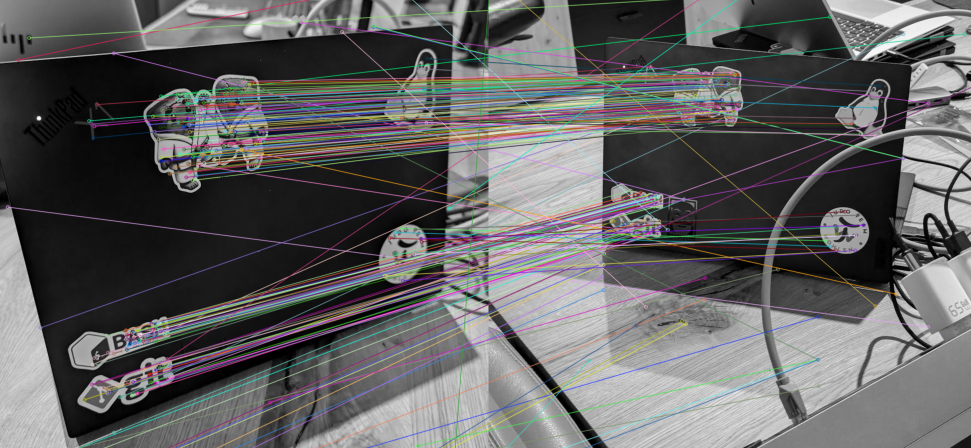
\includegraphics[width=1\linewidth]{assets/informatik-prototyp/opencv/sift/sift_good_example.png}
    \caption{Gutes Beispiel von SIFT Algorithmus}
    \label{fig:good-sift-example}
\end{figure}

Da unsere Objekte jedoch dreidimensionale sind und eine freie Rotation und Position in einem dredimensionalen Raum haben, ist es für den Algorithmus sehr schwierig Objektmerkmale festzulegen und diese in den verschiedenen Szenarien wieder zu detektieren:

\begin{figure}[H]
    \centering
\begin{subfigure}{1\textwidth}
    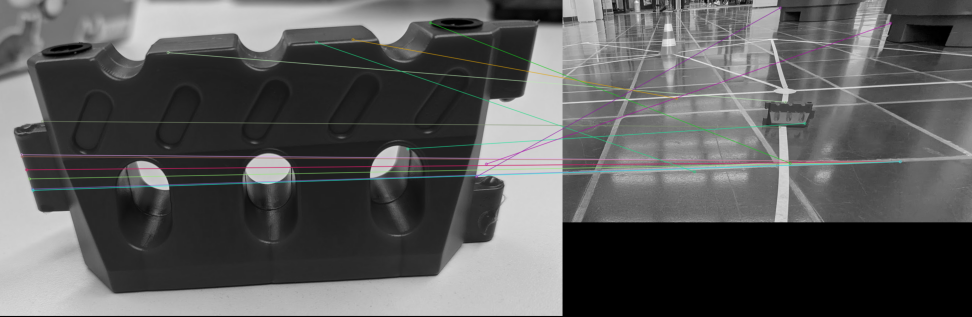
\includegraphics[width=1\linewidth]{assets/informatik-prototyp/opencv/sift/sift_our_usecase_example.png}
    \caption{SIFT Algorithmus}
    \label{fig:bad-sift-example}
\end{subfigure}
\begin{subfigure}{1\textwidth}
    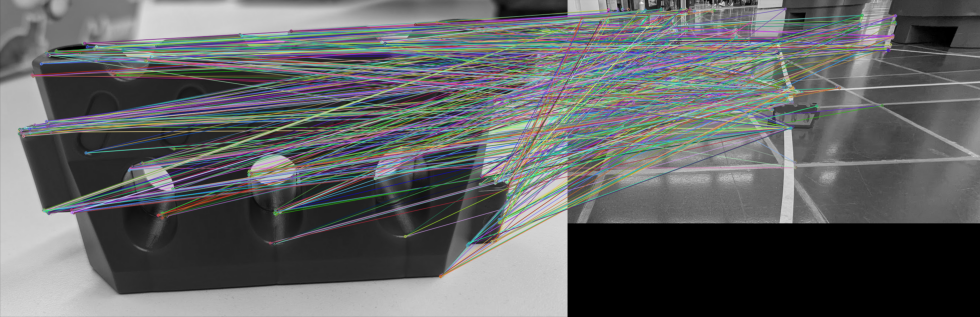
\includegraphics[width=1\linewidth]{assets/informatik-prototyp/opencv/sift/orb_our_usecase_example.png}
    \caption{ORB Algorithmus}
    \label{fig:bad-orb-example}
\end{subfigure}
    \caption{SIFT und ORB in unserem Usecase}
    \label{fig:sift-orb-in-our-usecase}
\end{figure}


Aus diesem Test können wir entscheiden, dass die OpenCV Merkmalsdetektionsalgorithmen nicht ausreichen, um Objekte in der 3D Umgebung sauber zu detektieren. Deshalb wird dieser Ansatz nicht mehr weiter verfolgt.

\textbf{Objekterkennung mit Farberkennung}

Grundsätzlich können Objekte auch nur rein durch ihre Farbe detektiert werden. Jedoch sind die Resultate stark von Umgebungsbedingungen abhängig.
Wir haben grundsätzlich 3 oder 4 verschieden Objekte zu Detektieren:
\begin{itemize}
    \item Pylone (Orange)
    \item Barriere (Rot)
    \item Barriere (Weiss)
    \item Knoten (Weiss)
\end{itemize}

Orange und rote Objekte können grundsätzlich sehr einfach detektiert werden. Da diese Farben in der Umgebung, wo der Roboter schlussendlich operiert, sehr eindeutig sind:

\begin{figure}[H]
    \centering
    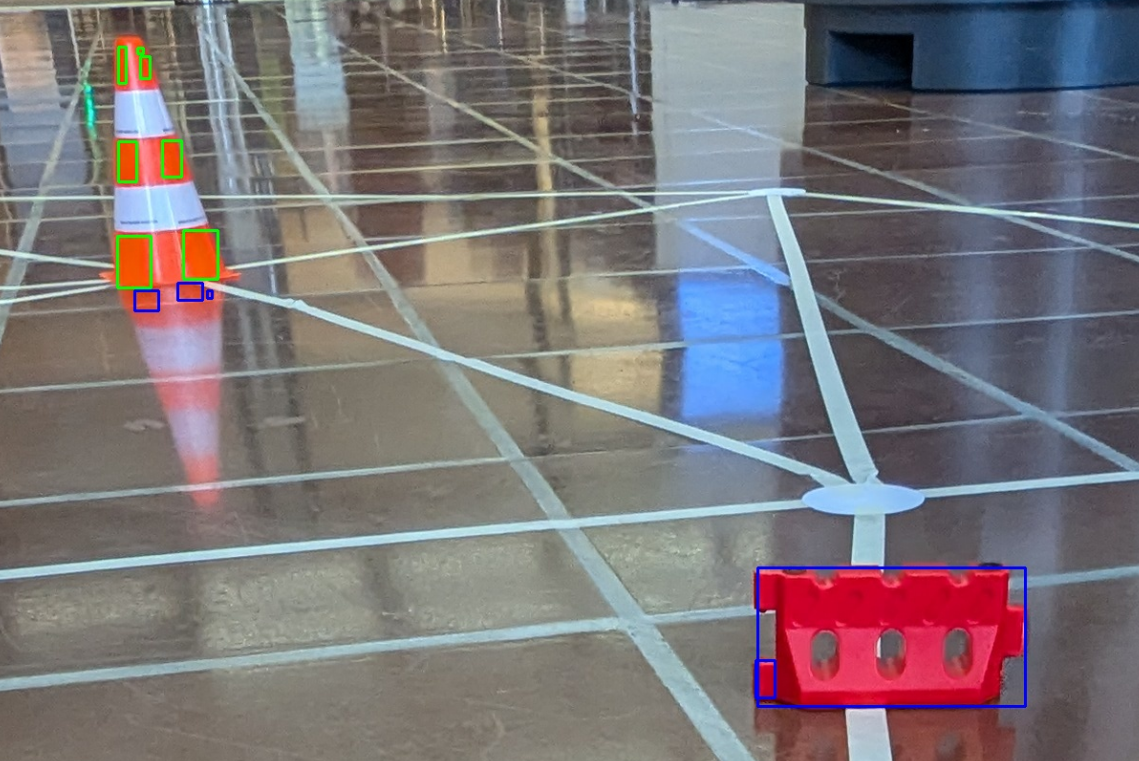
\includegraphics[width=0.5\linewidth]{assets/informatik-prototyp/opencv/object_detection_with_hsv/hsv_object_detection.png}
    \caption{Objekterkennung mittels Farberkennung der roten Barriere und orangen Pylone}
    \label{fig:opencv_hsv_object_detection_good}
\end{figure}


Die weisse Barriere und der weisse Knoten macht es jedoch schwieriger, denn einerseits haben sie die gleiche Farbe, was das unterscheiden dieser schwierig macht, und unter anderem haben wir, unter verschiedenen Lichtverhältnissen, Spiegelungen, welche sich im Bild auch als weisse Flecken darstellen und somit als Objekte erkennt werden:

\begin{figure}[H]
    \centering
    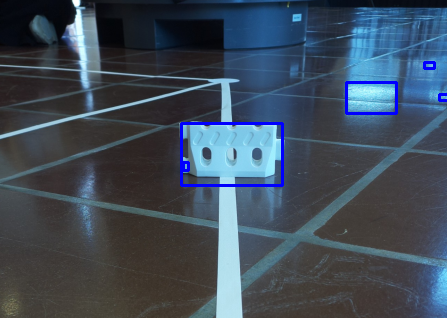
\includegraphics[width=0.5\linewidth]{assets/informatik-prototyp/opencv/object_detection_with_hsv/hsv_object_detection_white.png}
    \caption{Objekterkennung mittels Farberkennung der weissen Barriere}
    \label{fig:opencv_hsv_object_detection_bad}
\end{figure}

Mit vielen Feineinstellungen ist es eventuell auch möglich, die weissen Objekte zu detektieren. Jedoch ist es nicht eine sichere Lösung, da die Lichtverhältnisse in dieser Umgebung stark variieren und wir keine Kontrolle darüber haben.

\textbf{YOLOv11}

Auf Roboflow\footnote{https://roboflow.com/} wurden die insgesamt 58 erstellten Bilder gelabelt.
Das bedeutet, dass manuell die zu erkennenden Objekte ausgewählt und zu bestimmten Klassen hinzugefügt wurden.

Danach wird das Datenset unterteilt in verschiedene Gruppen: Train, Validation, Test. Die Training Daten werden verwendet mit den Markierungen, damit das Model davon lernen kann. Das Validierungsset wird benötigt, um während dem Trainingsprozess zu prüfen, wie gut das Model ist und wie es angepasst werden soll. Das Testset wird schlussendlich verwendet, um zu testen, wie gut das angepasste Model die einzelnen Elemente erkennt. Das Testset ist erforderlich, da die Daten, die zur Bewertung der Modellleistung verwendet werden, dem Modell vollständig unbekannt sein müssen.
\begin{figure}[H]
    \centering
    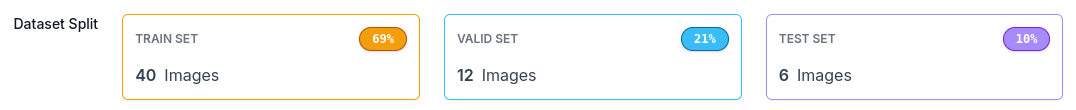
\includegraphics[width=\linewidth]{assets/informatik-prototyp/yolo/dataset-split.png}
    \caption{Datenset Split}
    \label{fig:data-split}
\end{figure}

Als erstes wurde versucht ein Model zu trainieren, das alle Graphenelemente (Knoten und Kanten) und Hindernisse erkennt:

\begin{figure}[H]
\begin{subfigure}{0.55\textwidth}
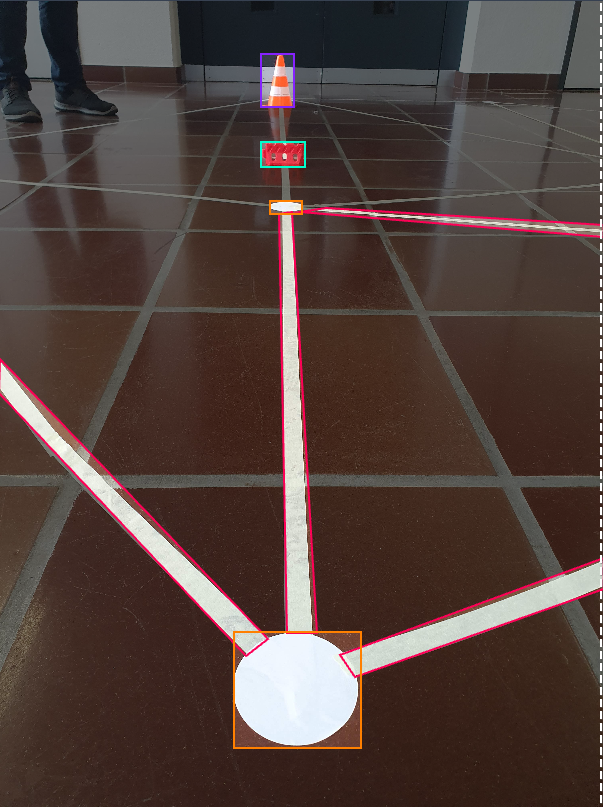
\includegraphics[width=0.95\linewidth]{assets/informatik-prototyp/yolo/labeled-image-lines.png} 
\caption{Bild mit Elementen + Linie markiert}
\label{fig:labeled-image-lines}
\end{subfigure}
\begin{subfigure}{0.4\textwidth}
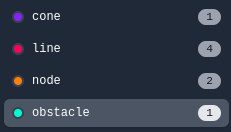
\includegraphics[width=0.95\linewidth]{assets/informatik-prototyp/yolo/labeled-classes-lines.png} 
\caption{Markierte Klassen mit Linie}
\label{fig:line-classes-lines}
\end{subfigure}

\caption{Roboflow labeled Bild mit Linien}
\label{fig:labeling-with-lines}
\end{figure}


Mihilfe eines Jupyter Notebooks, welches von Roboflow zur Verfügung gestellt wird, wurde ein YOLO Model mit 10 Epochs\footnote{\url{https://deepai.org/machine-learning-glossary-and-terms/epoch}} trainiert. Danach wurden Bilder aus dem Testset genutzt, in welchem das Model versucht die einzelnen Elemente zu erkennen. Zusätzlich wurde eine Confusion Matrix\footnote{\url{https://www.sciencedirect.com/topics/engineering/confusion-matrix\#:\~:text=A\%20confusion\%20matrix\%20represents\%20the,by\%20model\%20as\%20other\%20class.}} erstellt, die zeigt, welche Elemente als was erkannt wurde.

\begin{figure}[H]
\begin{subfigure}{0.3\textwidth}
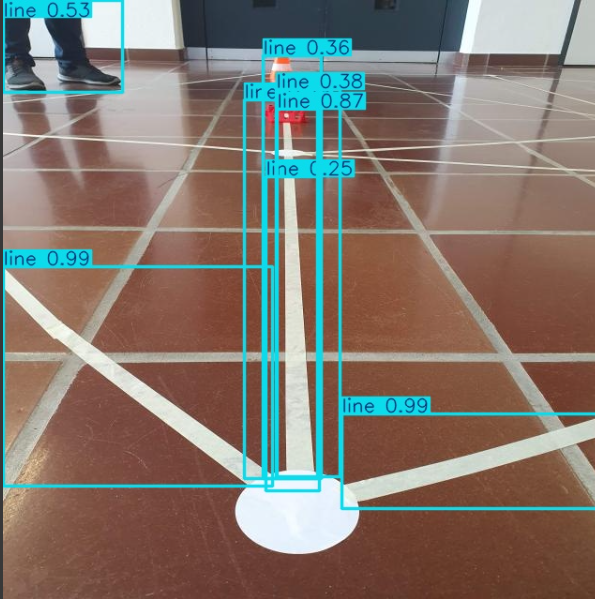
\includegraphics[width=0.95\linewidth]{assets/informatik-prototyp/yolo/line-recognitions.png} 
\caption{Erkanntes Bild mit Linien}
\label{fig:image-recognition-with-lines}
\end{subfigure}
\begin{subfigure}{0.69\textwidth}
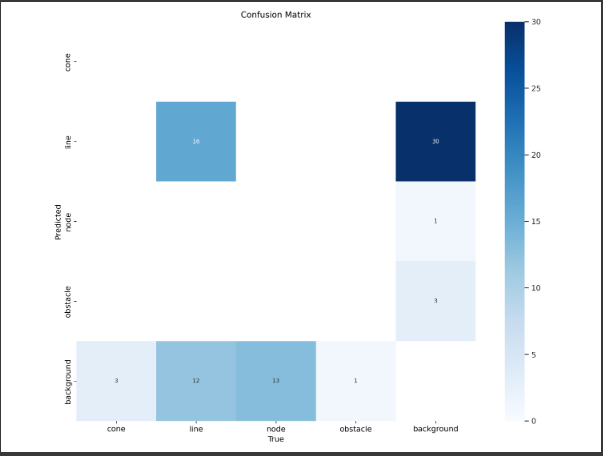
\includegraphics[width=0.95\linewidth]{assets/informatik-prototyp/yolo/conf-matrix-lines.png} 
\caption{Confusion Matrix mit Linien}
\label{fig:conf-matrix-lines}
\end{subfigure}

\caption{Bilderkennung inklusive Linien}
\label{fig:recognition-with-lines}
\end{figure}

Aus diesem Experiment war klar, sowohl aus dem Bild mit den "erkannten" Linien, als auch von der Confusion Matrix, dass Linien nicht korrekt erkannt werden können.
Aus der Confusion Matrix kann gelesen werden, dass von allen erkannten Linien in 4 Bildern, 30 Linien erkannt wurden an Stellen, an denen sich gar nichts befindet ("background").

Als nächstes wurde das gleiche noch einmal durchgeführt. Dieses Mal wurde die Line-Klasse entfernt und es wurden nur noch Knoten, Pylonen und Barrieren markiert.

\begin{figure}[H]
\begin{subfigure}{0.55\textwidth}
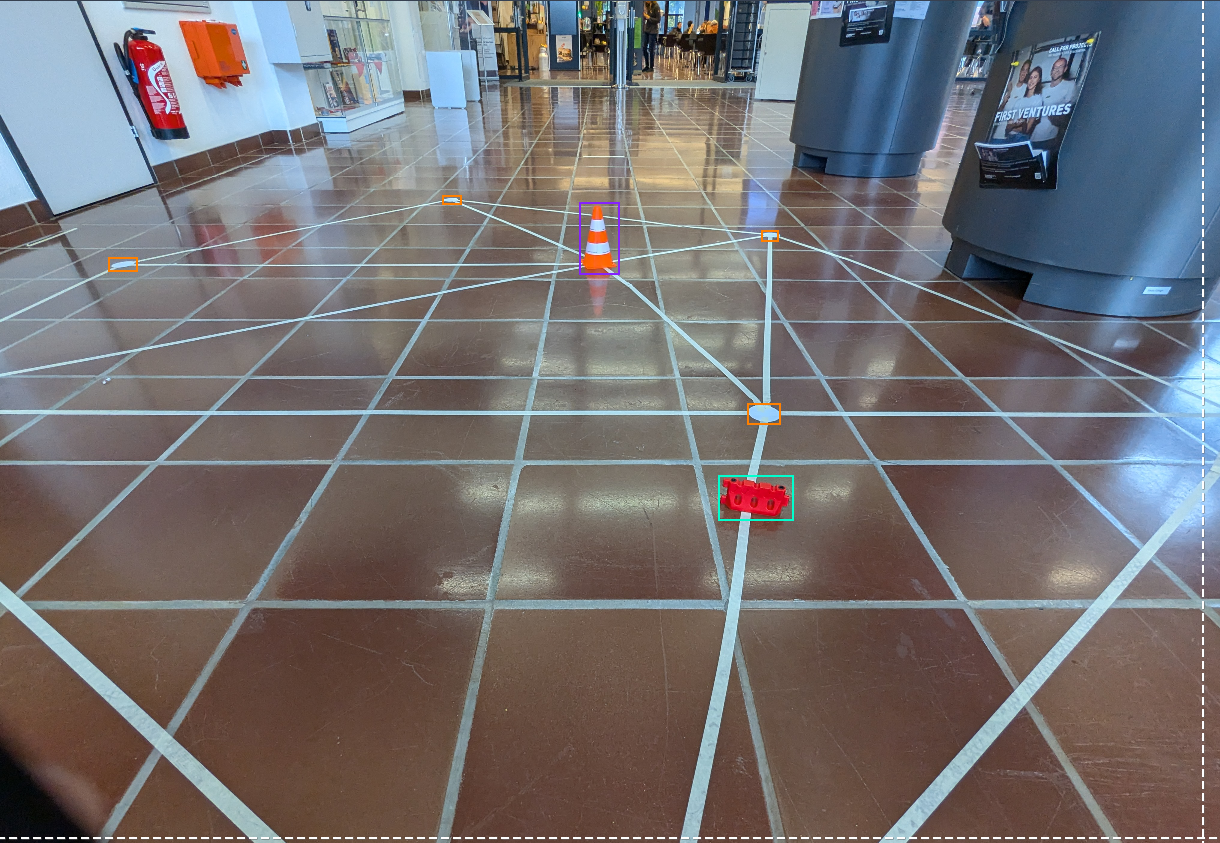
\includegraphics[width=0.95\linewidth]{assets/informatik-prototyp/yolo/labeled-image.png} 
\caption{Bild mit Elementen markiert}
\label{fig:labeled-image}
\end{subfigure}
\begin{subfigure}{0.4\textwidth}
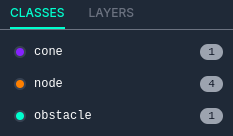
\includegraphics[width=0.95\linewidth]{assets/informatik-prototyp/yolo/labeled-classes.png} 
\caption{Markierte Klassen}
\label{fig:line-classes}
\end{subfigure}

\caption{Roboflow labeled Bild mit Linien}
\label{fig:labeled-with-lines}
\end{figure}

Die Bilderkennung des selben Jupyter Notebooks mit den reduzierten Klassen sah wie folgt aus:

\begin{figure}[H]
\centering
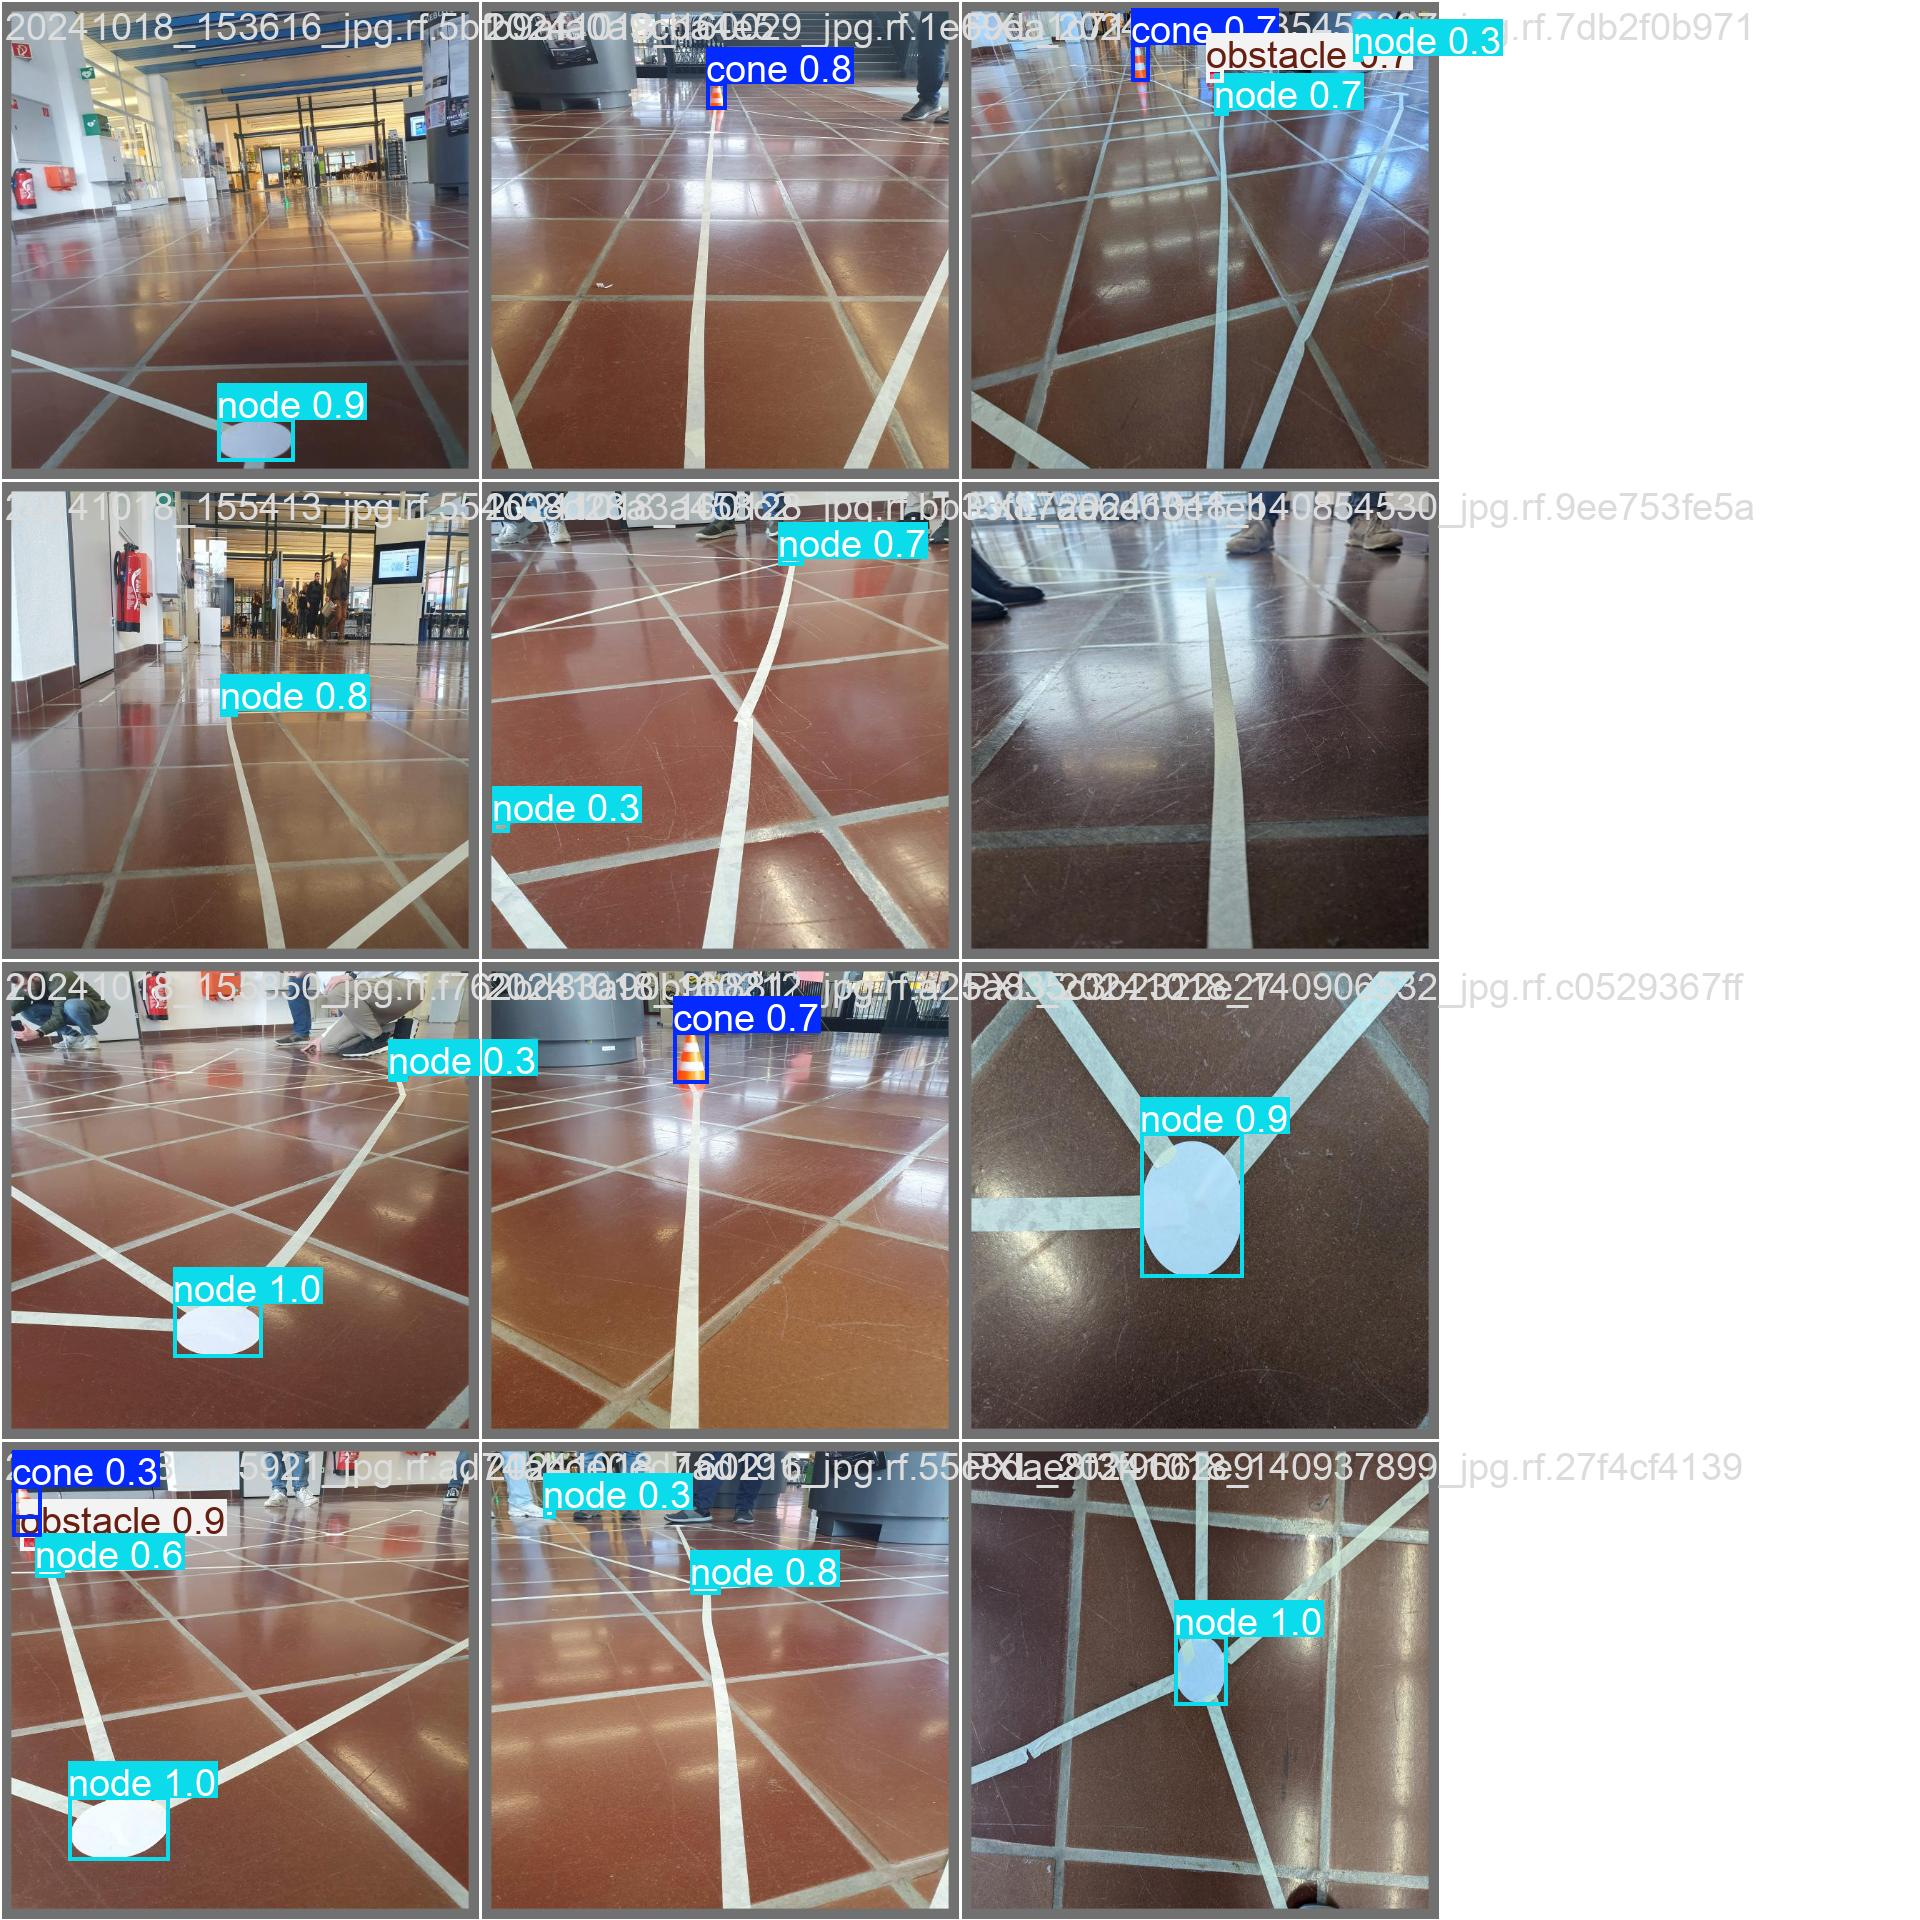
\includegraphics[width=\textwidth -30mm]{assets/informatik-prototyp/yolo/recognized-images.jpeg}
\caption{YOLOv11 Bilderkennung}
\label{fig:img-recognition-yolo}
\end{figure}

\begin{figure}[H]
\centering
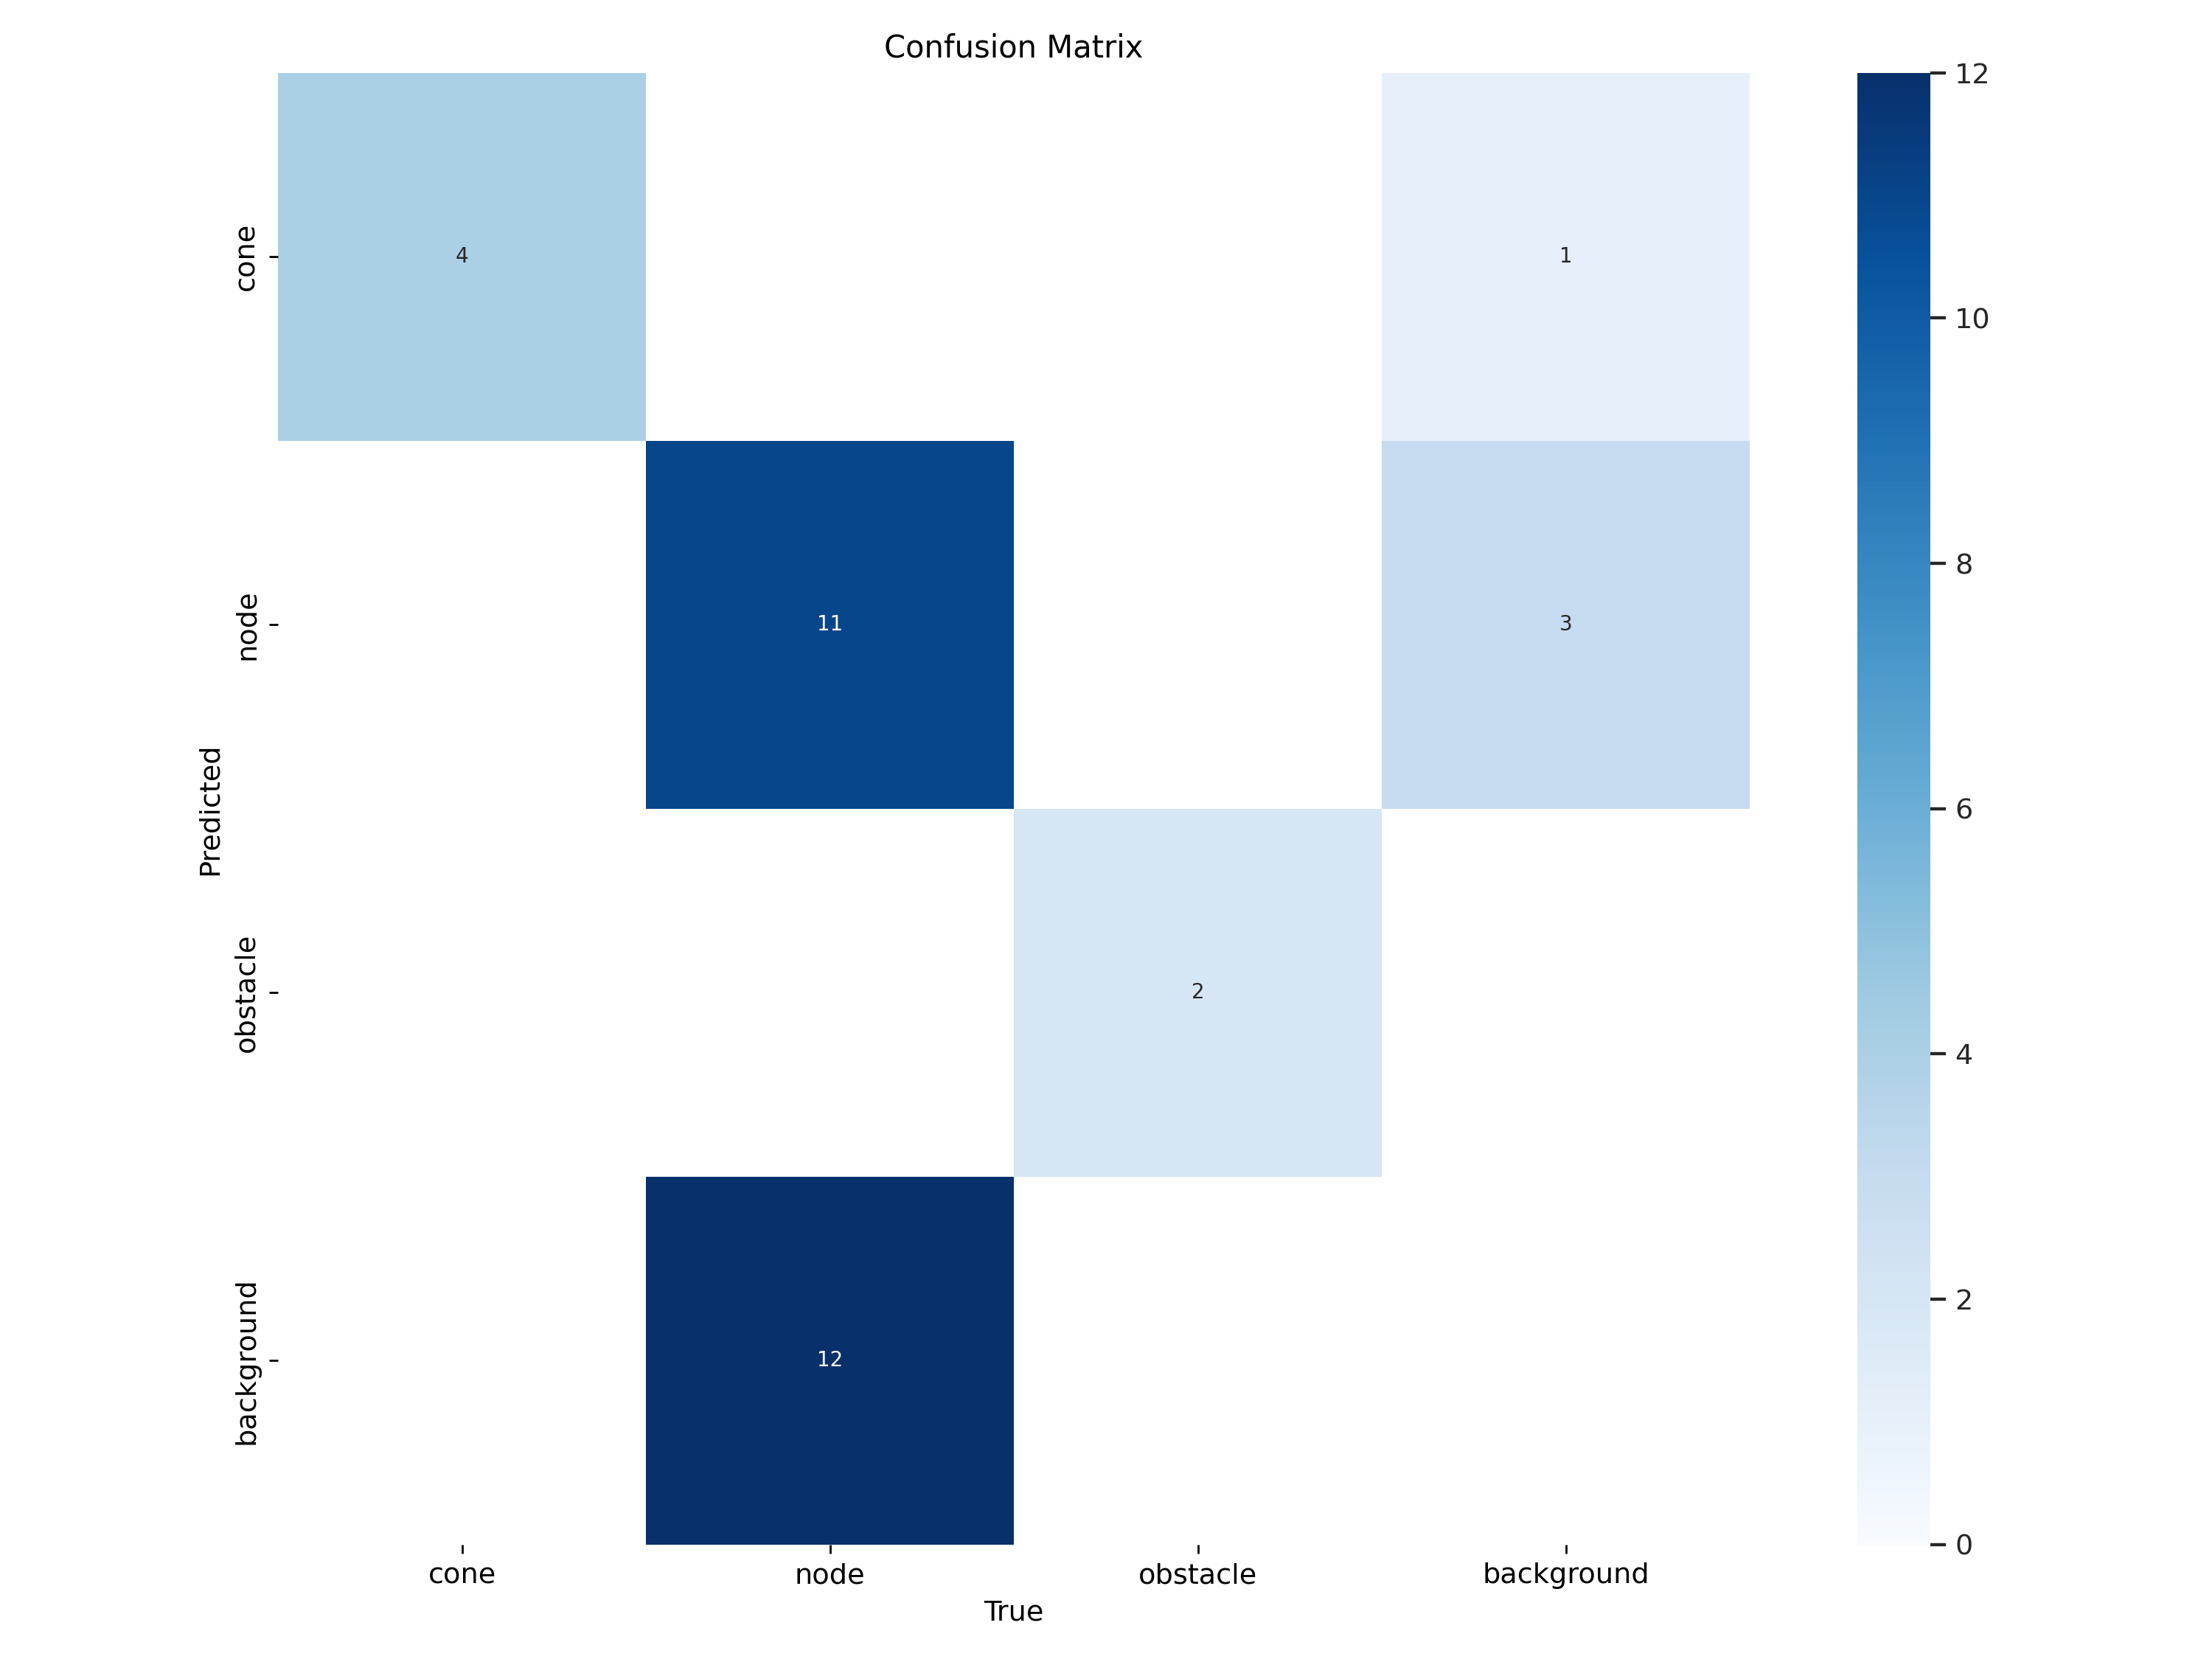
\includegraphics[width=\textwidth -20mm]{assets/informatik-prototyp/yolo/conf-matrix.png}
\caption{YOLOv11 Confusion Matrix Knoten, Barrieren und Pylonen}
\label{fig:conf-matrix-yolo}
\end{figure}

Aus dieser Matrix kann gelesen werden, dass alle Pylonen und alle Barrieren richtig erkannt werden. Einmal wird eine Pylone erkannt, obwohl es keine gibt. Die meisten vorausgesagten Knoten, sind wirklich Knoten, jedoch werden viele Knoten nicht erkannt. Dabei muss jedoch bedacht werden, dass es einfacher ist für das Model Knoten zu erkennen, die nahe und dadurch deutlicher sind und dass das Trainingsdatenset sehr klein ist. Trotzdem besteht ein sehr wahrscheinliches Risiko, dass ein Knoten nicht erkannt werden könnte.

Das gleiche Experiment wurde noch einmal durchgeführt mit nur Pylonen und Barrieren:

\begin{figure}[H]
\begin{subfigure}{0.55\textwidth}
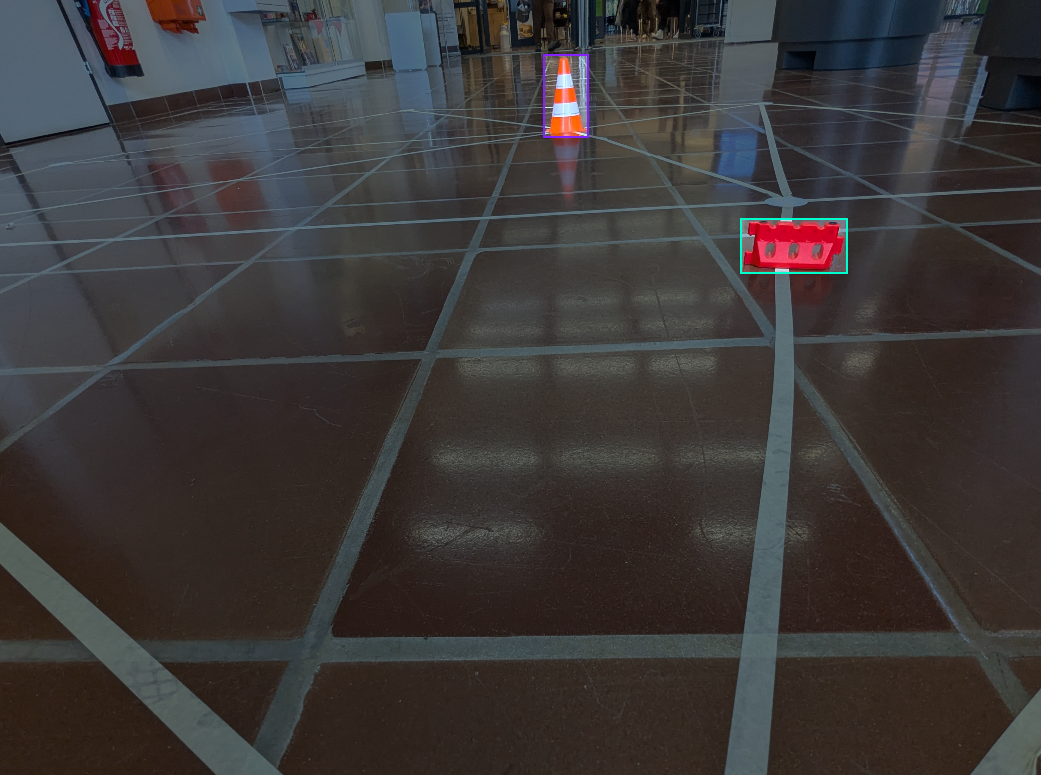
\includegraphics[width=0.95\linewidth]{assets/informatik-prototyp/yolo/label-cone-obstacle.png} 
\caption{Bild mit Hindernissen markiert}
\label{fig:labeled-image-obst}
\end{subfigure}
\begin{subfigure}{0.4\textwidth}
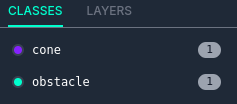
\includegraphics[width=0.95\linewidth]{assets/informatik-prototyp/yolo/classes-cone-obstacle.png} 
\caption{Markierte Klassen}
\label{fig:cone-obst-classes}
\end{subfigure}
\caption{Roboflow labeled Bild nur mit Hindernissen}
\label{fig:labeling-with-cone-obst}
\end{figure}


Die Resultate für die Pylonen und die Barrieren ist dasselbe, wie im vorherigen Experiment, jedoch fällt, wie erwartet die Unsicherheit der Knoten weg. Das Problem ist es nun, dass aus den erkannten Elementen auf dem dargestellten Bild geschlossen werden würde, dass sich auf dem nächsten Knoten ein Pylon befindet, da der vorherige Knoten nicht mehr erkannt wird.

\begin{figure}[H]
\begin{subfigure}{0.5\textwidth}
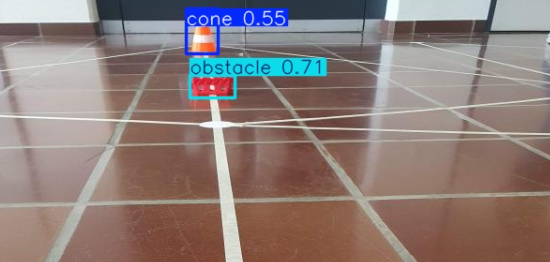
\includegraphics[width=0.95\linewidth]{assets/informatik-prototyp/yolo/cone-obst-recognition.png} 
\caption{Erkanntes Bild mit Hindernissen}
\label{fig:image-recognition-with-cone-obst}
\end{subfigure}
\begin{subfigure}{0.5\textwidth}
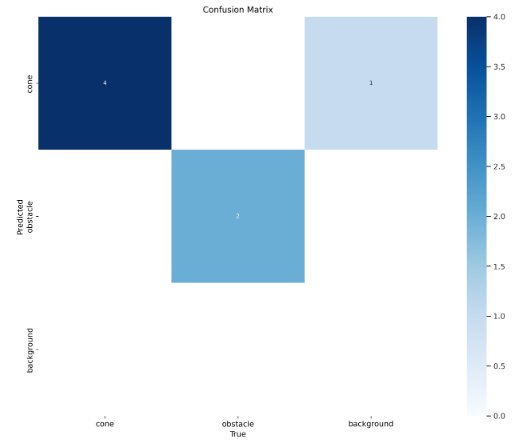
\includegraphics[width=0.95\linewidth]{assets/informatik-prototyp/yolo/cone-obst-conf-matrix.png} 
\caption{Confusion Matrix mit Hindernissen}
\label{fig:conf-matrix-cone-obst}
\end{subfigure}

\caption{Bilderkennung mit Hindernissen}
\label{fig:recognition-with-cone-obst}
\end{figure}



\textbf{Fazit}

Zur Erkennung der Hindernisse und des Graphens funktionierte YOLO am besten. Dabei wird versucht, die Hindernisse und die Graphenknoten zu erkennen. Die Unsicherheit der Knotenerkennung ist jedoch ein grosses Risiko. Deshalb wird eine Strategie verfolgt, die mit den ausgehenden Linien vom Knoten arbeitet und nur mit den anliegenden Knoten arbeitet.

\subsubsection{Zielknoten erkennen}

Der Roboter muss in der Lage sein, die Buchstaben auf den Zielknoten zu erkennen, um sicherzustellen, dass er sich wirklich im Ziel befindet. Dazu wurden drei verschiedene Varianten evaluiert: Tesseract OCR Algorithmus\footnote{\url{https://tesseract-ocr.github.io/}}, EasyOCR \footnote{\url{https://github.com/jaidedai/easyocr}} und \acrfull{orb}\footnote{\url{https://docs.opencv.org/4.x/d1/d89/tutorial_py_orb.html}}.

Die Tests wurden bei allen drei Varianten mit den folgenden drei Bildern durchgefuehrt. Diese sind unveraenderte Aussschnitte aus dem zur Verfuegung gestellten Muster der Zielknoten. Die Bilder wurden nicht pre-processed, da sie bereits in perfekter Qualitaet sind.

TODO they are all very different size

\begin{figure}[H]
\begin{subfigure}{0.3\textwidth}
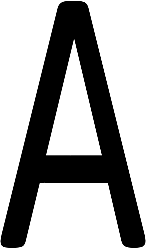
\includegraphics[width=0.95\linewidth]{assets/informatik-prototyp/opencv/target_node_detection/a.png} 
\caption{Muster A}
\label{fig:image-a}
\end{subfigure}
\begin{subfigure}{0.3\textwidth}
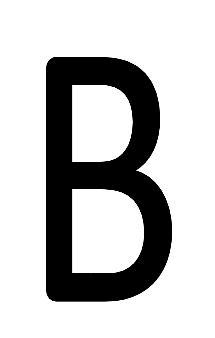
\includegraphics[width=0.95\linewidth]{assets/informatik-prototyp/opencv/target_node_detection/b.png} 
\caption{Muster B}
\label{fig:image-b}
\end{subfigure}
\begin{subfigure}{0.3\textwidth}
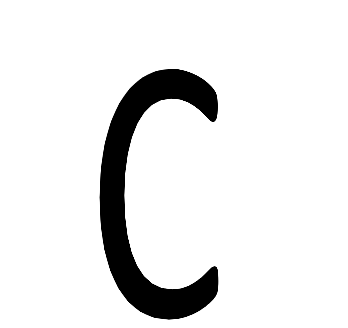
\includegraphics[width=0.95\linewidth]{assets/informatik-prototyp/opencv/target_node_detection/c.png} 
\caption{Muster C}
\label{fig:image-c}
\end{subfigure}

\caption{Muster der Zielknoten}
\label{fig:muster-zielknoten}
\end{figure}


\textbf{Tesseract OCR}

Tesseract ist ein bekannter Algorithmus, um Text zu lesen. Es gibt einen Modus, der sich darauf spezialisiert nur einzelne Buchstaben anstatt Textbloecke zu lesen. Dieser wurde bei dem Prototyping verwendet mit der Option \verb|--psm 10|. Ausserdem wurde festgelegt, dass nur die Buchstaben A, B und C erkannt werden koennen. Dies wurde wie folgt mit der Python Tesseract Bibliothek\footnote{\url{https://pypi.org/project/pytesseract/}} implementiert. 

\begin{verbatim}
text = pytesseract.image_to_string(image, config='--psm 10 -c tessedit_char_whitelist=ABC')
\end{verbatim}

Dabei konnte Tesseract ohne Probleme die Buchstaben A und C lesen, jedoch konnte der Buchstabe B nicht gelesen werden:

\begin{figure}[H]
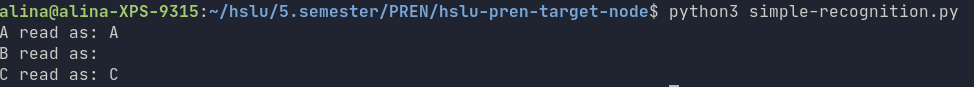
\includegraphics[width=0.95\linewidth]{assets/informatik-prototyp/opencv/target_node_detection/tesseract.png} 
\caption{Zielknotenerkennung mit Tesseract}
\label{fig:zielknoten-tesseract}
\end{figure}


\textbf{EasyOCR}

EasyOCR wird zur Extrahierung von Text verwendet. Da AI verwendet wird dazu, benoetigt dieser sowohl mehr Rechenpower, als auch mehr Zeit, die Bilder zu verarbeiten. Dieser Algorithmus ist Teil von der OpenCV Bibliothek. EasyOCR hat die Buchstaben wie folgt erkannt:

\begin{figure}[H]
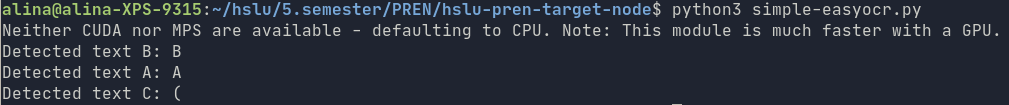
\includegraphics[width=0.95\linewidth]{assets/informatik-prototyp/opencv/target_node_detection/easyocr.png} 
\caption{Zielknotenerkennung mit EasyOCR}
\label{fig:zielknoten-easyocr}
\end{figure}

Bei EasyOCR sind zwei Probleme aufgetreten. Zum einen ist die Ausfuehrung des Algorithmus bereits auf einem Laptop recht langsam und zum anderen wird der Buchstabe C als Klammer-Auf \verb|(| erkannt.

\textbf{ORB}

\gls{orb-gloss} lernt die Merkmale von Objekten und erkennt auf einem Bild, welches Objekt gefunden wurde. Alle gfundenen Matches wurden in diesem Experiment nach Wahrscheinlichkeit sortiert. Mit diesem Verfahren konnten alle Knoten erkannt werden. Die Musterknoten wurden um 35 Grad gedreht, um zu pruefen, ob ORB auch Buchstaben erkennt, wenn sie nicht gleich rotiert sind, wie auf dem Muster Bild.

\begin{figure}[H]
\begin{subfigure}{0.3\textwidth}
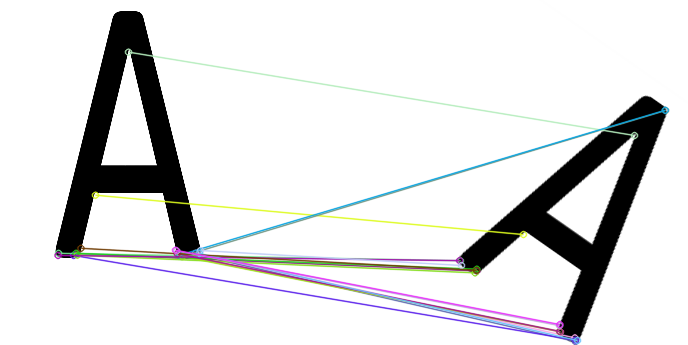
\includegraphics[width=0.95\linewidth]{assets/informatik-prototyp/opencv/target_node_detection/orb-a.png} 
\caption{ORB A}
\label{fig:orb-a}
\end{subfigure}
\begin{subfigure}{0.3\textwidth}
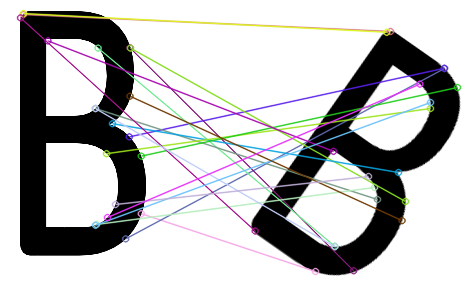
\includegraphics[width=0.95\linewidth]{assets/informatik-prototyp/opencv/target_node_detection/orb-b.png} 
\caption{ORB B}
\label{fig:orb-b}
\end{subfigure}
\begin{subfigure}{0.3\textwidth}
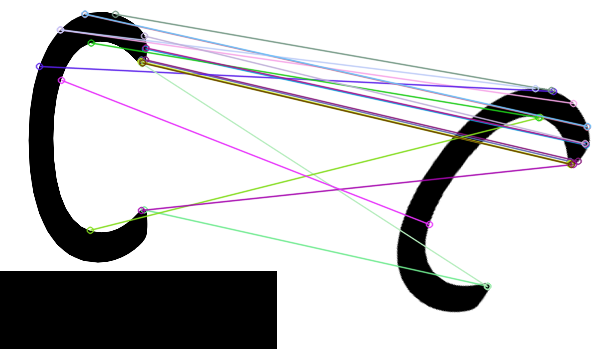
\includegraphics[width=0.95\linewidth]{assets/informatik-prototyp/opencv/target_node_detection/orb-c.png} 
\caption{ORB C}
\label{fig:orb-c}
\end{subfigure}

\caption{Zielknotenerkennung mit ORB}
\label{fig:orb-zielknoten}
\end{figure}

\textbf{Fazit}

Zur Erkennung der Buchstaben wird der \acrshort{orb} Algorithmus verwendet werden. Dieser hatte keine Probleme damit die Buchstaben klar zu erkennen und es werden sicher nur A, B oder C erkannt, da der Algorithmus nur diese Buchstaben kennt. Auf diese Weise kann verhindert werden, dass zum Beispiel 'C' als ein Klammer-auf \verb|(| gelesen wird. Ebenfalls ist keine Rotation des Bild des Zielknotens noetig, da ORB die Buchstaben auch rotiert erkennt.